\cleardoublepage

\section{背景和相关工作}

本章节我们对瞬态执行漏洞测试程序生成的相关背景和工作进行介绍。背景部分我们将会对 RISCV 指令集架构、
瞬态执行漏洞、处理器模糊测试尤其是差分模糊测试等技术进行介绍。在相关工作部分,我们则会对国内外瞬态执行漏洞挖掘
的测试程序生成、测试执行和漏洞检测等技术进行介绍。\par

\subsection{RISC-V指令集架构}

RISC-V 指令集架构(ISA)是一种开源的精简指令集架构\cite{riscv-isa-manual-all}。
它由一个基本的整数指令集和一组可选的指令集扩展组成。
标准扩展包含整数乘除法扩展(M)、内存原子操作扩展(A)、单精度浮点扩展(F)、双精度浮点扩展(D)和压缩指令扩展(C),等。
此外,控制和状态寄存器指令扩展(ZICSR)提供特权态管理功能, 而屏障指令扩展(ZIFENCEI)提供指令内存同步功能。\par

RISC-V 指令分为 32 位常规指令(包含六种指令格式)和 16 位的压缩指令(包含九种指令格式)两种。 
图\ref{review:base-inst}和图\ref{review:compress-inst}显示了所有 15 种指令类型的格式,
每种指令由多个字段组成。32 位指令的指令格式由 opcode 字段决定,而 16 位指令的格式由 op 和 funct 字段同时决定。\par

\begin{figure}[!h]
    \centering
    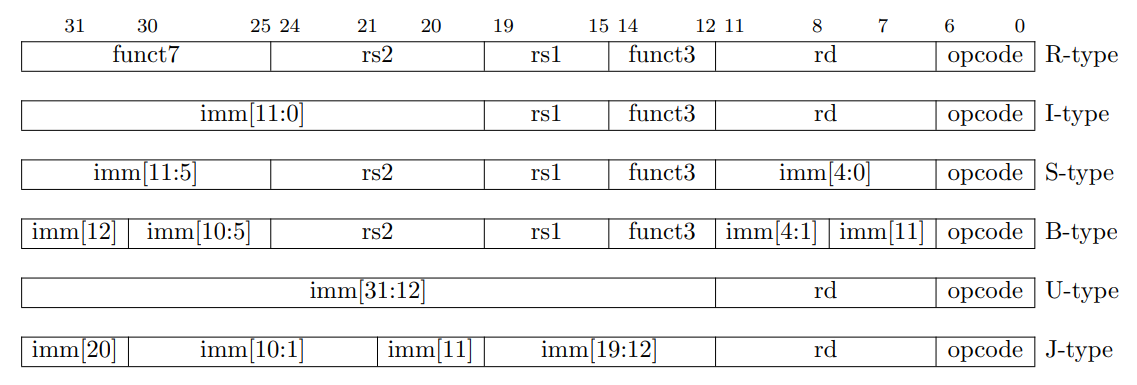
\includegraphics[width=\linewidth]{figure/proposal/riscv-base-instruct-format.png}
    \caption{RISCV基本指令格式}
    \label{review:base-inst}
\end{figure}
\begin{figure}[!h]
    \centering
    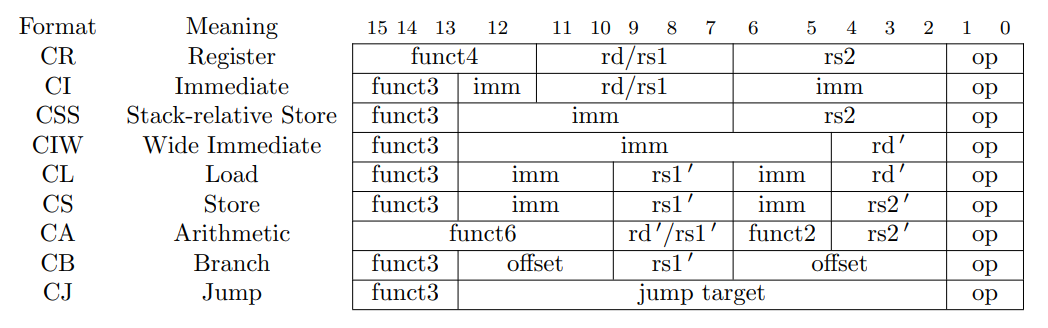
\includegraphics[width=\linewidth]{figure/proposal/riscv-compress-instruct-format.png}
    \caption{RISCV压缩指令格式}
    \label{review:compress-inst}
\end{figure}

指令字段可分为两类:
\begin{enumerate}
    \item 操作码相关字段,如 funct 和 opcode 字段。
opcode 字段和 op 字段的低 2 位用于确定指令的长度,而 funct 字段和 opcode 字段的其它位用于确定指令格式和功能。
通常,具有相似功能的指令有相同的 opcode 字段,并通过 funct 字段来区分具体功能。\par
    \item 操作数相关的字段,包括 imm,rs 和 rd 字段。
其中 rs 字段用于选择源寄存器,imm 字段用于表示立即数,rd 字段用于选择目的寄存器,即写回指令结果的寄存器。\par
\end{enumerate}

\subsection{瞬态执行攻击}
瞬态执行漏洞是现代处理器的关键漏洞。
现代处理器为了追求高性能,广泛采用乱序执行和投机执行等技术提高硬件利用率。
由于异常延迟处理和推测错误等原因,部分指令会被错误执行,虽然其执行结果会在后续被撤销,
并不会影响处理器架构层执行结果的正确性,但仍可能引起处理器微架构的状态变化。
攻击者可以通过侧信道跟踪微架构的状态变化,进而恢复出处理器内部的机密信息,这种攻击方式称为瞬态执行攻击。\par

瞬态执行攻击过程可以分为如下三个阶段。\par

\textbf{触发瞬态执行窗口:}
通过操纵控制流和数据流,可以人为创造异常延迟处理或者推测错误等场景,触发瞬态执行窗口,从而临时性的绕过软硬件的安全权限检查。
例如 Meltdown 类型利用了延迟的权限检查,如延迟对页表条目中的标志位的检查\cite{horn2018meltdown},
或对浮点寄存器权限的检查\cite{stecklina1806lazyfp},暂时绕过硬件原语的安全权限检查,瞬态执行后续的代码;
而 Spectre 类型\cite{kocher2020spectre} 则通过毒害返回地址堆栈\cite{maisuradze2018ret2spec}、分支预测器等,
操纵控制流进入错误预测的跳转地址,从而暂时绕过软件的安全权限检查,瞬态执行错误预测地址之后的代码。\par

\textbf{访问秘密数据:}
在第一阶段触发瞬态执行窗口之后,处理器可以临时性的绕过软硬件的安全权限检查,执行没有安全权限的代码。
通过执行这些代码可以直接或者间接访问内存中的秘密数据,将秘密数据暂时从存储部件泄漏到寄存器中\cite{van2019ridl}\cite{van2021cacheout}。
这里可以直接访问秘密数据的地址,将内存、缓存、load buffer 中的秘密数据泄漏到寄存器中;
也可以访问低位对齐等相关的地址,将存储层次中的秘密数据泄漏到寄存器。

\textbf{使用侧信道泄露秘密数据:}
将秘密数据带入寄存器之后,通过微体系结构的微架构状态对秘密数据进行编码。
之后通过特殊的微架构跟踪技术,通过时间侧信道等侧信道,将编码在微架构状态中的秘密数据解码出来,从而实现秘密数据的侧信道泄露。
已知的瞬态执行漏洞往往通过缓存\cite{yarom2014flush+}、分支预测器\cite{evtyushkin2018branchscope}、
执行端口\cite{bhattacharyya2019smotherspectre}等微架构部件进行秘密数据的编码,
然后通过时间侧信道将编码在其中的信息泄露出来。
随着 CPU 复杂度的不断提高和瞬态攻击研究的不断推进,更多微架构状态和侧信道被用于瞬态攻击的执行。\par

\subsection{处理器模糊测试}

模糊测试一种自动化的测试技术,它会根据一定的规则自动或者半自动地生成随机数据,
然后输入到动态运行的被测程序入口,通过监控被测程序是否有异常情况发生(如系统崩溃,断言失败等)来发现存在的软件缺陷。
同时一些模糊测试生成器会根据被测程序插桩的信息反馈,有指向性的对输入数据进行突变,
进一步提高异常触发的效率和提高程序测试的覆盖率。
随着处理器复杂程度的提高,传统的处理器验证方式效果开始不断受限,
研究人员转而将模糊测试技术引入到处理器正确性验证领域 
\cite{bruns2022efficient}\cite{canakci2021directfuzz}\cite{hur2021difuzzrtl}。\par

处理器模糊测试和软件模糊测试一样也由三个阶段组成:\par

1.输入生成阶段:
模糊器使用种子生成指令流,并根据前一轮的覆盖范围对指令流进行突变,
如 DifuzzRTL\cite{hur2021difuzzrtl}使用静态分析技术生成指令,
而 TheHuzz\cite{kande2022thehuzz} 则使用最优权重优化算法进行突变。\par

2.硬件仿真阶段:
模糊测试工具使用硬件插桩技术来收集当前输入的覆盖率,现有的模糊测试工具设计了多种覆盖度量,
诸如 mux 覆盖\cite{laeufer2018rfuzz}、控制寄存器覆盖\cite{hur2021difuzzrtl}和硬件行为覆盖\cite{kande2022thehuzz} 等。\par

3.状态验证阶段:
模糊测试工具提取 DUT 的架构状态,然后将其与参考模型(例如,ISA 模拟器)进行比较,其中不匹配的行为将被标记为 bug。\par

\par

\textbf{差分模糊测试:}
差分测试需要一种检测机制来检测错误或者说检测异常行为。
虽然一些简单的错误如内存损坏、段错误等很容易被检测器捕获,但那些难以定义明确异常行为的语义错误则很难被检测到。
因此,差分测试被用于识别语义相关的 bug(如文件系统\cite{min2015cross}、JVM\cite{chen2019deep} 等),
它通过比较具有相同功能和执行目标的多个程序的执行结果进行错误检测,
如果这些程序显示不同的输入-输出关系,则可以认定这是一个bug。\par

瞬态执行漏洞因其语义的复杂性,难以用简单的逻辑约束进行表征和检测,
而差分测试正好适用于语义相关 bug 的识别,故而也被广泛运用于瞬态执行漏洞的检测。
具体方法如下:将两个仅秘密数据部分不同的可执行程序交给两个同样的处理器进行执行,如果两者执行的时间存在差异,
则可以认为可以通过时间侧信道对秘密数据进行泄露。\par

\subsection{国内外相关工作}

瞬态指令漏洞的 模糊测试 检测作为处理器 模糊测试 的变体,可以类似的分为输入生成阶段、测试执行阶段和漏洞检测阶段三部分。
本章节将从这三个方面分别进行研究方向和研究进展的介绍。

\subsubsection{输入生成}
输入生成阶段负责生成尝试触发瞬态执行漏洞的测试程序。\
早期的硬件 模糊测试 工具如 DifuzzRTL\cite{hur2021difuzzrtl}、
TheHuzz\cite{kande2022thehuzz}等基本采用纯随机的方式进行测试指令的生成,
处理器漏洞挖掘效率相对较低。为了进一步提高测试程序的质量,Razzle\cite{razzle}、
Cascade\cite{soltcascade}等工具会对程序的控制流进行约束,以此提高程序执行的覆盖率;
SpecDoctor\cite{hur2022specdoctor}等工作对指令的数据流进行了约束,
通过提高相邻指令的数据依赖,提高其在处理器微架构执行时的难度。\par

为了充分利用瞬态执行漏洞的语义特点,一些测试程序生成工具采用基于模板突变的方法,
试图高效的产生瞬态执行漏洞的变体。如Transynther\cite{moghimi2020medusa}是专注于 MDS 变体生成的工具,
它使用已知的MDS构建块和微代码进行组合,来构造新的 MDS 泄漏,
而SpeechMiner \cite{xiao2019speechminer}则专注于 Meltdown 变体的生成。
但这种方法可能会导致漏洞同质化,缺乏挖掘全新漏洞的能力。\par

\subsubsection{测试执行}

测试执行阶段负责让后端处理器执行前端生成的测试程序,尝试在执行中触发瞬态执行漏洞。
早期的工作会直接使用真实的处理器硬件执行测试程序,但是随着RTL漏洞检测重要性的提高,
基于RTL仿真的瞬态漏洞测试执行工作,如IntroSpectre\cite{ghaniyoun2021introspectre}、
SpecDoctor\cite{hur2022specdoctor}等开始兴起。
Verilator\cite{snyder2013verilator}等开源工具为RTL仿真提供了条件,
且在仿真的场景下还可以进行硬件插桩,便于后续阶段的漏洞检测。\par

但为了提高测试执行的效率,一些工作如Revixor\cite{oleksenko2022revizor}、
Scam-V\cite{nemati2020validation}、
Speculation at Fault\cite{hofmann2023speculation}等会对处理器硬件建立形式化模型,
然后基于形式化模型进行测试执行,其中Revixor\cite{oleksenko2022revizor}支持 x86 指令,
Scam-V\cite{hofmann2023speculation}支持 arm 指令,
Speculation at Fault\cite{hofmann2023speculation}则是对Revixor\cite{oleksenko2022revizor}
在异常相关类型漏洞上的一个补充。此外基于模型的测试方式也可以对模型直接进行瞬态执行漏洞的静态分析,
如UPEC\cite{fadiheh2020formal}根据开源RTL手动建立有界模型,然后利用静态分析的技术寻找瞬态漏洞。

\subsubsection{漏洞检测}

漏洞检测阶段负责对测试执行的结果进行分析,进而判断是否触发了瞬态执行漏洞。
差分测试是广泛使用的瞬态执行漏洞检测的方法,Revixor\cite{oleksenko2022revizor}、
Speculation at Fault\cite{hofmann2023speculation}等工作都使用差分测试进行瞬态执行漏洞检测,
SpecDoctor\cite{hur2022specdoctor}更是在两个不同的阶段分别运用了差分测试。\par

此外还可以用基于约束的方法进行瞬态执行漏洞的检测,如Transynther\cite{moghimi2020medusa}、
IntroSpectre\cite{ghaniyoun2021introspectre}通过检查缓冲区执行前后的变化进行漏洞检查,
SpeechMiner\cite{xiao2019speechminer}通过测量竞争条件判断漏洞的可用性。\par

差分测试和约束判断的漏洞检测方法有时还需要硬件插桩的辅助。
如果拥有 RTL 的源码,就可以通过 RTL 硬件插桩的方法为检测程序得到处理器内部的状态信息和事件信息,
甚至可以在处理器内存内嵌约束判断的电路逻辑,在测试执行的同时直接进行漏洞约束的判断。

\cleardoublepage
\section{研究挑战}

在生成瞬态执行漏洞的测试程序的时候,生成框架会遇到三个重要挑战。
首先,在指令生成层面,
生成框架生成的指令需要得到满足特定条件的操作数和指令间依赖,
以满足特定的数据流和控制流约束;
其次,为了高效地生成能触发瞬态窗口的代码,
生成框架需要有意识地为触发瞬态窗口的指令设计和排布训练代码;
最后,为了生成有效的测试程序,生成框架需要让程序的各个语义部分可以相互适配,
协同工作,因此生成框架需要根据语义对测试程序代码块进行合理划分和针对性生成,
然后将各阶段代码块有效组合起来,最终删除冗余代码,得到精简的测试程序。\par

\subsection{带约束的指令生成}
\textbf{约束指令操作数}。
为了触发瞬态执行漏洞,生成框架生成的指令需要能执行特定的操作。
例如为了可以泄露秘密数据或者触发内存访问异常,
访存指令计算得到的操作数需要落在特殊的内存地址范围内;
为了让控制流指令可以跳转到预设的地址,跳转指令计算得到的跳转地址需要等于预设的地址、
分支指令操作数的值要满足对应的比较规则等。
为了确保指令在执行时可以得到满足要求的操作数,从而实现特殊的语义行为(如跳到特殊地址、访问特殊内存等),
在生成指令时需要对指令立即数字段、数据段值、指令组合等进行约束处理。\par

\textbf{约束指令字段}。
为了触发一些预设的特殊场景,生成框架也需要对生成指令的字段进行约束。
例如为了增加指令间的数据流依赖,触发更复杂的流水线执行情况,需要对指令间的 rs、rd 等字段进行约束;
为了可以跳转到特定的地址、访问特殊的内存,需要对指令和数据的 label 等进行约束。\par

\subsection{瞬态窗口训练的生成}
\textbf{训练代码的生成}。
Spectre 等瞬态执行漏洞指出,触发瞬态窗口除了需要触发瞬态窗口的 trigger 指令(如 Spectre 的控制流指令、
Meltdown 的内存访问指令等),还需要有指令序列对 trigger 相关的微架构部件进行微架构状态的训练。
但是以往的工作如DifuzzRTL\cite{hur2021difuzzrtl}、TheHuzz\cite{kande2022thehuzz}、
SpecDoctor\cite{hur2022specdoctor}都是用随机代码生成的方式进行瞬态窗口触发代码的生成,
并没有有针对性地生成训练代码,这导致了瞬态窗口的生成效率低下。
故而生成器需要能根据 trigger 指令,有针对性地生成用于训练的指令序列,进而提高瞬态窗口触发的可能性。\par

\textbf{地址敏感的代码排布}。
指令序列对 trigger 的训练效果是地址敏感的。在多数情况下,训练指令只有在特殊的地址上才可以对 trigger 指令对应的微架构状态进行有效训练 。
例如对于 BOOM 处理器\cite{celio2017boomv2}的 branch 指令,
低地址对齐的控制流指令可以对该 trigger 对应的分支预测器表项进行有效训练,
从而将 branch 指令涉及的微架构调整到位。
为此,生成框架在生成训练代码的时候需要寻找合适的指令排布位置,
从而提高训练的成功率。 \par

\subsection{完整程序的生成}

\textbf{程序的模块分割}。
已知完整的瞬态执行漏洞程序由触发瞬态窗口、访问秘密数据、侧信道泄露秘密数据三部分代码组成,
为了提高生成框架对瞬态执行程序语义的利用,生成框架可以将三阶段代码进行进一步细分,并赋予每个
阶段更精确的功能语义,然后根据各个代码块的功能提供更有针对性的生成策略。\par

\textbf{程序的组合}。
为确保分割后的代码能够按场景依次执行、协同工作,从而组成完整有效的瞬态漏洞程序,
我们需要通过总结分析各个代码块之间的协作约束关系,包括操作数关系、控制流关系等,
设计出通用的代码组装模版,在确保瞬态漏洞程序有效运行的同时,尽可能多地覆盖各类瞬态漏洞场景。\par

\textbf{程序的精简}。
生成器得到的瞬态执行漏洞程序不可避免地包含了许多对瞬态执行攻击没有帮助的指令,
这些指令会增加程序模拟执行、漏洞检测时的时间开销,并且也会对后续定位程序中的漏洞带来负担。
因此生成框架需要使用合适的算法精简掉冗余的指令,从而得到精简的瞬态漏洞程序。\par

\cleardoublepage
\section{测试程序生成框架的设计}

本生成框架是一种针对 RISCV 处理器 RTL 的、用于瞬态漏洞查找的测试程序生成框架。
对于给定的 RISCV 处理器 RTL 和代码生成配置,该生成框架可以根据瞬态执行漏洞各阶段的程序特点,
高效地生成瞬态执行漏洞测试程序,寻找发动瞬态执行攻击的具体 PoC,进而准确的复现漏洞。 \par

\subsection{生成框架概述}

为了高效地生成有效的瞬态执行攻击程序,我们的生成框架分两阶段进行测试程序生成。
在阶段1中,生成框架生成触发瞬态窗口的指令序列,并在处理器 RTL 上检验该部分指令的有效性;
阶段2在阶段1成功的基础上,生成访问秘密数据和利用侧信道传递秘密数据的指令序列,
如果该指令序列在处理器上存在差分测试差异,即可得到能触发瞬态执行漏洞的完整 PoC。\par

\subsection{阶段1:触发瞬态窗口}

不同于 SpecDoctor 先生成能触发瞬态窗口的随机指令序列,再确定 trigger 指令和瞬态窗口位置;
我们的生成框架预先确定待触发的瞬态窗口和触发该瞬态窗口的 trigger 指令,再为 trigger 指令生成协同工作
的训练代码和其他代码。之后该测试程序会在 vcs 或者 verilator\cite{snyder2013verilator} 生成的处理器 RTL 上模拟执行,
检查预设的瞬态窗口是否触发。如果触发成功,生成框架会删去冗余的训练指令,然后进入阶段2生成后续指令。\par

\subsubsection{瞬态窗口触发代码的生成与排布}

为了实现触发瞬态窗口的目的,生成框架会生成如下配合工作的的代码块:\par

\textbf{全局初始化块(init块):}
init 块负责在程序执行伊始为所有特权寄存器赋初值,然后执行后续的瞬态窗口触发代码。\par
\textbf{退出块(exit块):}
exit 块负责 RTL 仿真程序的结束,当瞬态窗口测试代码执行完毕后进入 exit 块退出程序。\par
\textbf{寄存器初始化块(load\_init块):}
load\_init 块负责为后续所有被执行的块所使用的通用寄存器和浮点寄存器提供随机的初值或者传递指定的参数。\par
\textbf{延迟块(delay块):}
delay 块在 load\_init 块初始化之后执行,它由一系列强数据流依赖的多周期指令组成,用于延迟得到操作数的计算结果。\par
\textbf{触发块(trigger块):}
trigger 块负责触发瞬态窗口,紧接着 delay 块开始执行。为了延迟得到 trigger 指令的执行结果,
迫使处理器执行预测执行,trigger 指令的操作数需要依赖于 delay 块的计算结果。
此外,为了可以让 trigger 指令可以访问特殊的地址触发异常、或者跳转到非瞬态窗口的地址,生成框架会对 trigger 指令的操作数值进行约束,
确保地址访问或者地址跳转符合预期。\par
\textbf{瞬态窗口块(trans块):}
trans 块包含一个确保可以侧信道泄露秘密数据的默认指令序列,用于填充预设的待触发的瞬态窗口区域,
如果该部分的代码被瞬态执行,则预示着瞬态窗口被触发成功,该代码块退出到 exit 块。\par
\textbf{返回块(return块):}
return 块作为控制流指令类型的 trigger 块正确执行后跳转到的无害代码,该代码退出到 exit 块。\par
\textbf{空操作块(nop 块):}
nop 块被放置在 load\_init\_train 块和 delay 块之间,用于排空流水线,防止 delay 块、trigger 块在执行的过程中被 load\_init 块的内存访问指令的执行所影响。\par
\textbf{异常块(trap块):}
trap 块作为异常触发类型的 trigger 块正确执行后跳转到的无害代码,该代码退出到 exit 块。\par

其中 init 块、return 块、exit 块、trap 块是因为测试框架需要所涉及的,因此称为功能块(function 块);
load\_init 块、nop 块、delay 块、trigger 块用于瞬态窗口的触发,因此称为触发块(trigger 块);
trans 块暂时填充阶段二用于秘密数据泄露部分的代码的位置,因此属于泄露块(leak 块)。
根据瞬态漏洞触发的场景不同,生成框架用四种方式将上述代码块组织起来,如图\ref{paper:trigger-dist-situation}所示:\par

\textbf{场景一:} trigger 块的 trigger 指令是控制流指令,例如 branch、jmp 等,
预设的瞬态窗口紧接着 trigger 块排布,而 trigger 的跳转目标位于 trans 块之后的 return 块位置。
当程序正确执行时,trigger 的跳转指令会发生跳转进入 return 块然后进入 exit 块退出程序;
当程序前端预测部件预测错误,认为 trigger 指令不发生跳转或者跳转地址是紧挨着 trigger 块下一条指令时,
控制流会临时进入 trans 块进行瞬态执行。该情况可以囊括 spectre 的部分场景。\par

\textbf{场景二:} trigger 块的 trigger 指令是控制流指令(例如 branch、jmp 等),
或者不触发异常的顺序执行指令(例如 add、mul 等),
预设的瞬态窗口和 trigger 块不相邻,而 trigger 不发生跳转或者跳转目标紧接着 trigger 块。
此时可以让 return 块紧挨着 trigger 块排布,而 trans 块位于 return 块之后。
当程序正确执行时,trigger 的指令会进入 return 块然后进入 exit 块退出程序;
当程序前端预测部件预测错误,认为 trigger 指令发生跳转且跳转地址位于 trans 内部时,
控制流会临时进入 trans 块进行瞬态执行。该情况可以囊括 spectre 的部分场景。\par

\begin{figure}[!h]
    \centering
    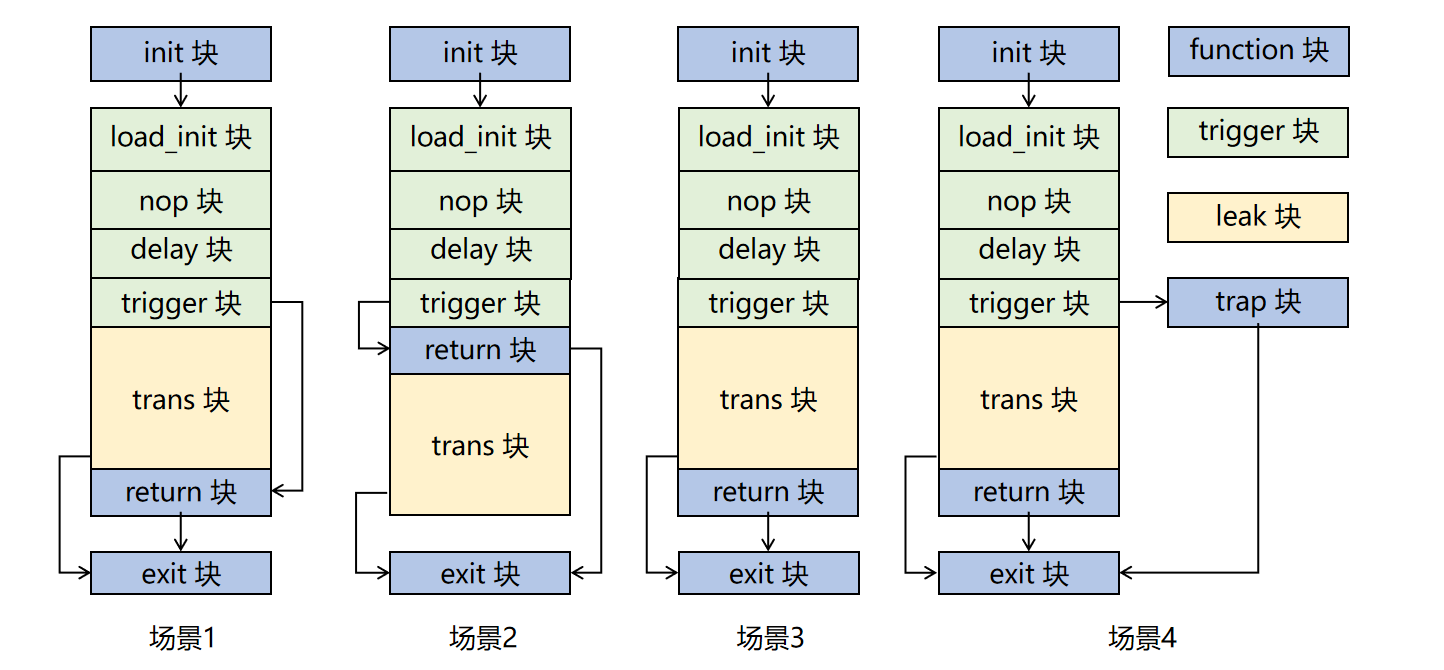
\includegraphics[width=\linewidth]{/mnt/d/txt/zjuthesis/figure/paper/arrange-stage1-situation.png}
    \caption{瞬态窗口触发代码块布局场景}
    \label{paper:trigger-dist-situation}
\end{figure}

\textbf{场景三:} trigger 块的 trigger 指令是 store 指令且修改 trans 块内部对秘密数据访问的地址时,
预设的瞬态窗口紧接着 trigger 块排布。当程序正确执行时,控制流进入了 trans 块,但是因为
秘密数据访问的地址被修改,使得秘密数据没有发生泄漏,之后进入 exit 块退出程序。
但是如果存在内存访问预测错误的情况,则会触发瞬态窗口,导致 trans 块会暂时用原先的秘密数据访问地址泄露秘密数据。
该情况可以囊括 spectre-V4 的场景。\par

\textbf{场景四:} trigger 块的 trigger 指令是触发异常的指令(例如 ecall、load、store 等),
预设的瞬态窗口紧接着 trigger 块排布。当程序正确执行时,
trigger 的指令触发异常进入 trap 块,然后进入 exit 块退出程序;
如果存在异常延时检查等情况,则 trigger 块后续的 trans 块的指令会继续被顺序执行,触发瞬态窗口。
该情况可以囊括 meltdown 的部分场景。\par

对上述场景适当合并和化简之后,代码的执行和排布顺序如图\ref{paper:trigger-dist}所示,首先执行 init 块,
然后顺序排布和执行 load\_init 块、nop块、delay 块、trigger 块。
根据 trigger 指令的指令类别,决定后续排布的 return 块和 trans 块的顺序。trap 块位于其他位置,在异常发生的时候进入。
最后 return 块、trans 块、trap 块都会跳转进入 exit 块结束硬件模拟程序。这里的 load\_init 块、delay 块、trigger 块、nop 块
trans 块、return 块组成了一个完整的指令组合,我们称之为 victim group。\par

\begin{figure}[!h]
    \centering
    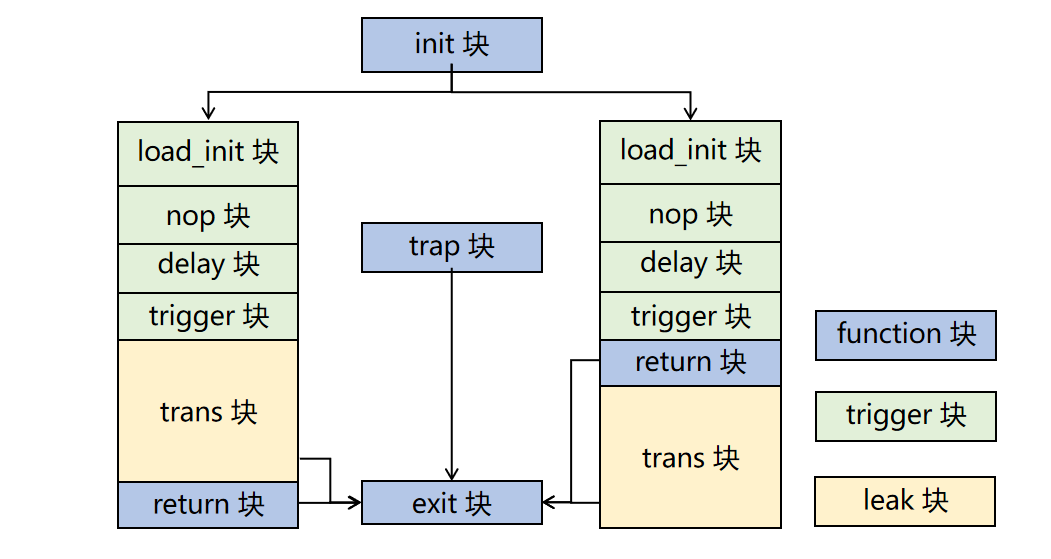
\includegraphics[width=0.8\linewidth]{figure/paper/arrange-stage1.png}
    \caption{瞬态窗口触发代码块布局}
    \label{paper:trigger-dist}
\end{figure}

\subsubsection{训练代码的生成和排布}

为了 trigger 块的 trigger 指令可以更有效地触发瞬态窗口,生成框架需要生成额外的 train 指令对 trigger 指令进行训练,
因此生成框架在之前的基础上引入了用于训练的 train 块。train 块可以由单条或者多条任意类型的指令随机组合得到,
对于 train 块中的控制流指令和内存访问指令,生成框架对跳转地址和访问地址做额外约束,确保程序能正确执行。\par

考虑到 trigger 指令相关部件的微结构状态训练是地址敏感的,
因此 train 块布局的地址最好有和 trigger 的地址相关,如虚拟地址、甚至物理地址相同或者地址低位对齐等。
为了达到最高效的训练效果,也为了对物理地址空间和虚拟地址空间做最小的改动,
硬件额外扩展了一种物理内存切换机制,可以硬件中对物理地址对应的内存单元直接进行切换,
从而确保 train 块和 trigger 块可以先后在同一物理地址执行,进而提高 train 块训练成功的概率。\par

为了实现充分多种类的训练功能,生成框架将会生成如下代码块:\par

\textbf{训练初始化块(load\_init\_train 块):}
load\_init\_train 块用于初始化 train 块需要的通用寄存器和浮点寄存器,提供随机值或者满足约束条件的特殊值,
该部分代码和 victim group 的 load\_init 块共享物理地址空间。\par

\textbf{训练块(train 块):}
train 块用于对 trigger 块的 trigger 指令设计的微架构状态进行调整,
该部分代码和 victim group 的 trigger 块共享物理地址空间

\textbf{空操作块(nop 块):}
nop 块被放置在 load\_init\_train 块和 train 块之间,
用于填充 train 块和 load\_init\_train 块之间的部分。\par

\textbf{返回块(return 块):}
同触发瞬态窗口的 return 块,用于作为 train 块中跳转指令的可选跳转目标,
和 victim group 的 return 块共享物理地址。\par

\textbf{空返回块(nop\_return 块):}
nop\_return 块用于填充 victim group 的 trans 块的位置,用于作为 train 块中跳转指令的可选跳转目标。
该代码块可以跳转到内存切换代码地址,兼具 nop 块和 return 块的功能。\par

对于已生成的 victim group 指令序列,生成框架会生成对应地址布局的训练代码。这部分训练代码由上述的
load\_init\_train 块、nop 块、train 块、nop\_return 块、return 块组合而成,我们称之为 train group。
因为 train group 的 load\_init\_train 块、train 块的长度和 victim group 的 load\_init 块、trigger 块的长度
存在差异,为了确保它们的起始地址或者结束地址可以对齐,需要对 nop 块的长度进行调整。\par

有时候一个 train group 并不能有效训练 victim group,因此生成框架会依概率为 victim group
生成一系列 train group,依次执行,来提高成功训练 trigger 指令的可能性。
如图\ref{paper:memory-switch},当执行测试程序时,
首先执行第一个 train group 的指令序列,然后返回到物理内存切换的指令部分,
执行物理内存切换,物理内存的指令切换为下一个 train group 继续训练,直到最后切换为
被训练的 victim group 开始尝试触发瞬态窗口。\par

\begin{figure}[!h]
    \centering
    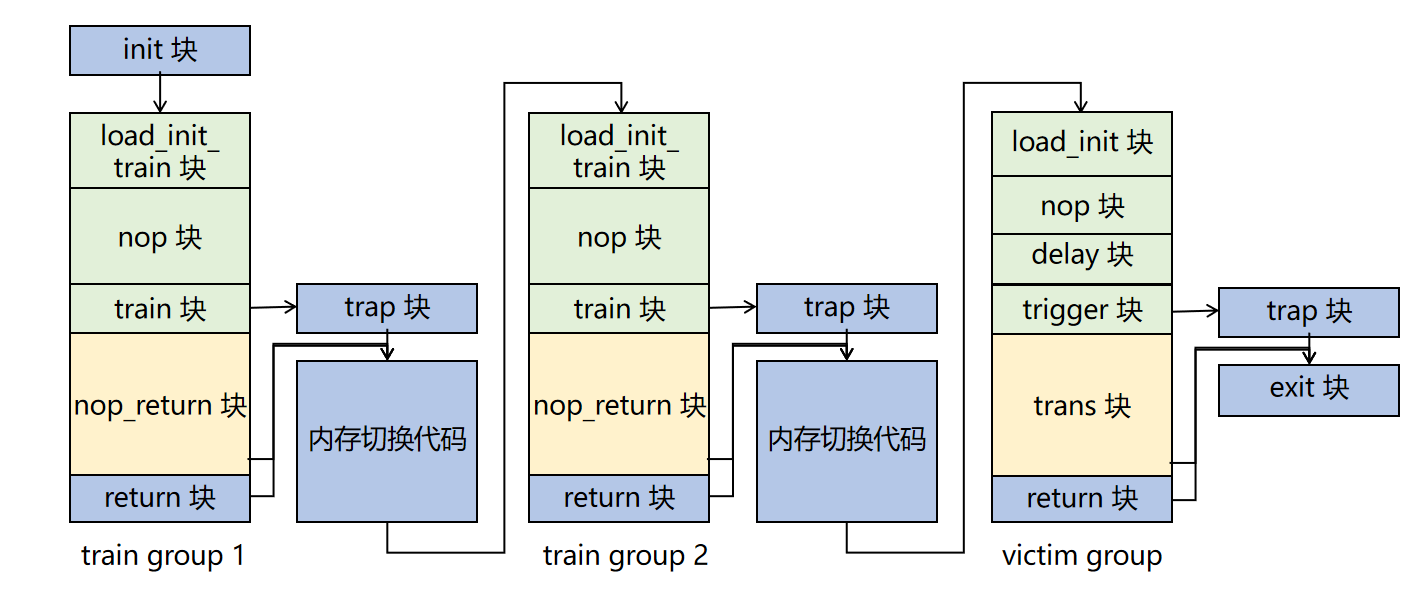
\includegraphics[width=\linewidth]{figure/paper/group-switch.png}
    \caption{代码组内存切换}
    \label{paper:memory-switch}
\end{figure}

\subsubsection{瞬态窗口触发检验}

为了判断阶段一生成的代码能否有效执行,生成框架生成的测试程序
需要在 vcs 或者 verilator 编译生成的处理器 RTL 上模拟执行,
检测是否触发了瞬态窗口,也即是否执行了 victim group 的 trans 块的代码。\par

为此生成程序预留了一组\textbf{slti zero, zero, imm}的指令作为 label 指令,用于标志特殊的指令事件的发生。
并会在 trans 块内部生成特殊的 label 指令表示瞬态执行窗口的开始(这里使用 INFO\_TEXE\_START 作为 label 指令)。
之后我们对处理器的 rob 模块进行插桩,如果发现 label 指令进入 rob 和从 rob 中提交,就保存对应的 log 到指定文件。
如果 INFO\_TEXT\_START 指令进入 rob 的次数多于从 rob 中提交的次数,就说明 INFO\_TEXT\_START 在瞬态窗口中被执行了,
也即测试程序可以成功触发瞬态窗口,阶段一代码生成成功。

\subsubsection{测试程序的简化}

在为 victim group 生成 train group 序列的时候,测试框架为了确保 trigger 指令被有效训练,
可能会生成过饱和的 train group 序列。其中有部分 train group 可能是无效的,或者冗余的。
为了减轻后续阶段二执行 train group 的开销,也为了更好的定位训练 trigger 指令的有效 train 片段,
生成框架需要能删去多余的 train group 代码。\par

\begin{algorithm}[!h]
    \caption{Train Simplificaiton}
    \label{alg:TS}
    \renewcommand{\algorithmicrequire}{\textbf{Input:}}
    \renewcommand{\algorithmicensure}{\textbf{Output:}}
    
    \begin{algorithmic}[1]
        \REQUIRE train group list $train\_list$, vicitm group $victim$  %%input
        \ENSURE train group list after simplificaiton $new\_train\_list$    %%output
        \STATE $new\_train\_list \Leftarrow train\_list$
        \FOR{each $i \in [1, len(train\_list)]$}
            \FOR{each $j \in [1, len(new\_train\_list)$]}
                \STATE $tmp\_train\_list \Leftarrow new\_train\_list with new\_train\_list(i)$
                \IF{$trigger_test(tmp\_train\_list, victim) == True$}
                    \STATE $new\_train\_list \Leftarrow tmp\_train\_list$
                    \STATE \textbf{break}
                \ENDIF
            \ENDFOR
        \ENDFOR

        \RETURN $new\_train\_list$
    \end{algorithmic}
\end{algorithm}

生成框架使用算法\ref{alg:TS}进行 train group 的简化。该算法尝试删去 train group 序列中的一个 train group,
然后重新执行处理器模拟执行,如果仍然可以触发瞬态窗口,尝试删除下一个 train group。
如果尝试删除任意一个的 train group 之后都无法触发瞬态窗口,则化简结束,得到局部最优的 train group 序列。\par

\subsection{阶段2:访问和泄露秘密数据}

在阶段1得到的触发瞬态窗口代码的基础上,生成框架继续生成访问秘密数据和利用侧信道传递秘密数据的代码,
并通过处理器差分测试检测生成的测试程序能否最终触发瞬态执行攻击。
如果测试存在执行时间的差异,该测试程序即为完整的瞬态执行攻击的 PoC。

\subsubsection{访问秘密数据代码的生成与排布}

为了实现访问秘密数据的目的,生成框架会生成如下的代码块:\par

\textbf{秘密数据访问块(access\_secret 块):}
access\_secret 块的代码会生成待泄露的 secret 数据的地址,然后用 load 指令访问该内存,
将 secret 数据读取到寄存器中。生成的地址可以和秘密数据地址完全相同,也可以只是和秘密数据地址低位对齐的,
以尝试挖掘处理器潜在的 MDS 内存地址匹配漏洞。因为访问秘密数据的过程只能在瞬态执行的过程中进行,
因此 access\_secert 块的代码需要被布局在 trans 块的内部。\par

\textbf{秘密数据迁移块(migrate\_secret块):}
migrate\_secret 块负责转移 secret 数据在分层存储结构中的位置。处理器内存采用load缓冲区、cache、memory
的多层次存储结构,access\_secret 块的不同数据访问方式对不同深度的存储单元的访问能力是不同的,
因此生成框架需要产生秘密数据迁移的代码,将秘密数据迁移到合适的存储深度,提高 access\_secret 块
成功访问秘密数据的能力。migrate\_secret 仅使用其他块没有使用的寄存器进行操作,因此不会影响其他寄存器的执行结果。\par

\begin{figure}[!h]
    \centering
    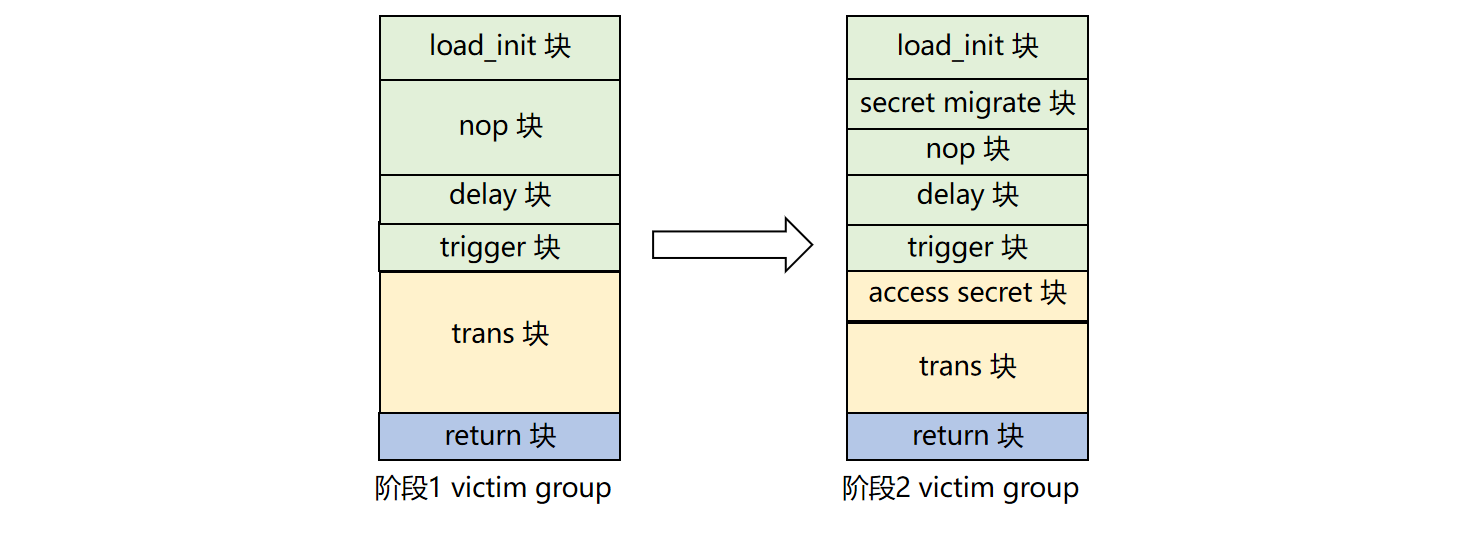
\includegraphics[width=\linewidth]{figure/paper/stage2-access-secret.png}
    \caption{访问秘密数据代码的排布}
    \label{paper:access-secret}
\end{figure}

如图\ref{paper:access-secret},
这两部分代码在阶段2会被组装进入 victim group。对于 access\_secret 块,
因为访问秘密数据的过程只能在瞬态执行的过程中进行,
因此 access\_secert 块的代码需要被布局在 trans 块的内部;
而对于 migrate\_secret 块,这部分代码虽然可以在瞬态窗口外部被执行,
但是在执行了 migrate\_secret 块的指令之后应该尽可能的避免内存访问指令的执行,
以防破坏 secret 在内存结构中的位置,因此这部分代码被放置在 load\_init 块之后,delay 块之前。
故而阶段2首先会根据随机配置,生成 access\_secret 块和 secret\_migrate 块,
并将原先的 victim group 调整为如图的布局。\par

当 victim group 的代码被执行时,程序在执行完 load\_init 块的寄存器初始化之后,
就会执行 secret\_migrate 块的代码将秘密数据迁移到处理器存储结构的合适位置,然后执行后续代码触发瞬态窗口。
瞬态窗口被触发之后,access\_secret 块被执行,试图将 secret\_migrate 块迁移之后的秘密数据
从存储层次结构读取到寄存器中。\par

\subsubsection{侧信道泄露代码的生成与排布}

为了实现侧信道泄露秘密数据的目的,生成框架会生成如下的代码块:\par

\textbf{编码块(encode 块):}
encode 块尝试利用 access\_secret 块访问得到 secret 数据修改处理器的微架构状态,
以此实现将 secret 数据编码到处理器微架构状态的目的。为了让 encode 块有较强的 secret 数据传播和编码能力,
生成的指令会尽可能多的使用 secret 数据,并让生成的指令之间存在较强的数据竞争和结构竞争。\par

\textbf{解码块(decode 块):}
decode 块尝试利用 encode 产生的微架构状态差异产生执行时间上的差异,
以此实现将 secret 在处理器微架构的编码利用时间侧信道解码的目的。
因为重复执行相同的指令会涉及到相同微架构部件的使用,故而一条指令被重复执行时,
其执行结果易受初次执行时产生的微架构状态的影响,
因此生成框架简单使用和 encode 块相一致的代码作为 decode 块。\par

\textbf{替换块(replace 块):}
replace 块用于替换 encode 块和 delay 块之间的部分,它直接用立即数指令生成 secret 数据的值,并将值存储到和 access\_secret 一致的目的寄存器中。
执行 replace 块可以得到和 access\_secret 块一样的执行结果,但是并不会修改 cache、内存等存储单元。

在进行代码排布时,encode 块需要在瞬态窗口中执行,因此被放置在 trans 块内部,且在 access\_secret 块执行完毕后执行;
decode 块为了可以和 encode 块使用尽可能一样的处理器部件,因此它除了指令和 encode 块高度相似外,
还需要地址和 encode 块保持一致,因此生成框架新定义一个 decode group,
将 decode 块排布在 decode group 中与 encode 块相同的物理地址处。\par

\begin{figure}[!h]
    \centering
    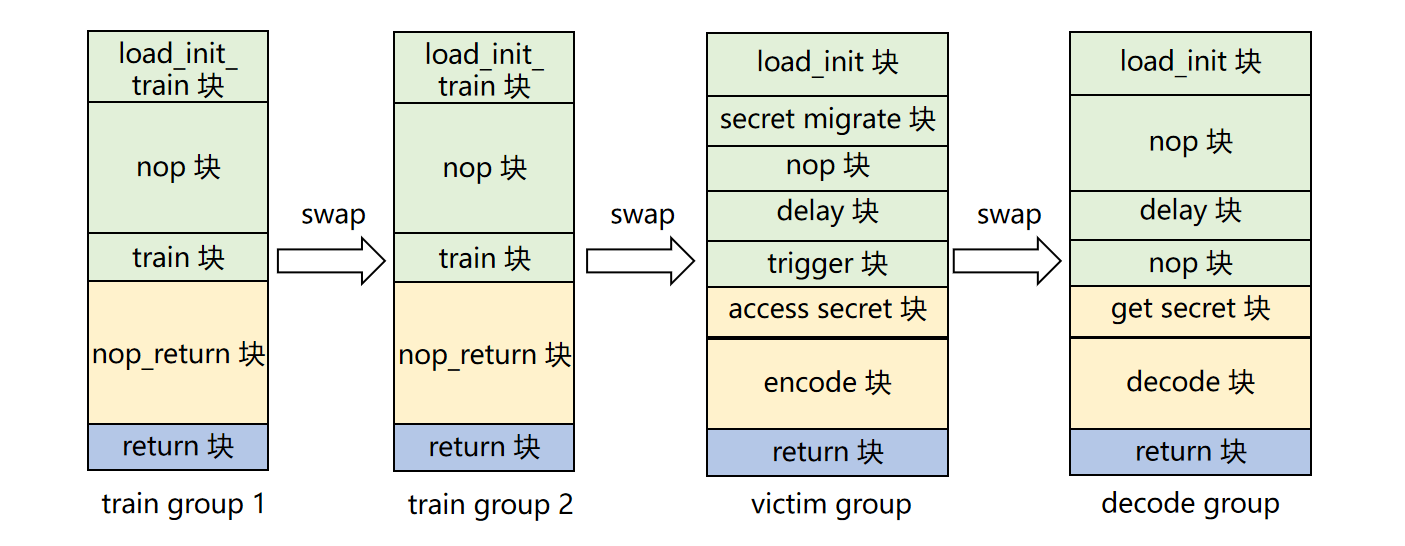
\includegraphics[width=\linewidth]{figure/paper/group-switch-all.png}
    \caption{完整程序内存切换}
    \label{paper:group-switch-all}
\end{figure}

decode group 在 victim group 之后执行,用于对 encode 块编码在处理器中的 secret 数据进行解码。
如图\ref{paper:group-switch-all}所示,完整程序在执行时首先执行 train group 序列进行 trigger 指令的训练,
然后切换到 victim group 触发瞬态窗口、访问秘密数据和将秘密数据编码到微架构状态,最后切换到 decode group,
尝试从微架构状态中解码 secret 的值。为了确保 decode group 执行 decode 块时可以获得和 encode 块执行时一样的操作数,从而使用一样的处理器部件,
decode group 复制 victim group 的 load\_init 块、delay 块;secret\_migration 块用 nop 块替代;
trigger 块、access\_secret 块和两者之间可能存在的 return 块用 replace 块代替,避免修改cache、内存的状态;decode 块替代 encode 块。
因此 decode group 最后的代码块排布如图\ref{paper:group-switch-all}中的 decode group 所示。\par

\subsubsection{秘密数据泄露检验}

我们采用差分测试的方法对测试程序是否发生瞬态执行漏洞攻击进行检验,如图\ref{paper:differential-test}所示。
首先将上述的所有 group 和其他框架代码导出为完整的测试程序,在处理器 RTL 上模拟执行。
为了测量测试程序的执行时间,生成框架会在程序结尾插入特殊 label 指令,
然后对 RTL 进行内部插桩,当该 label 指令被执行时 dump 此时的处理器周期数。
之后将测试程序的 secret 部分替换掉,再次进行模拟执行和 dump 执行结束时的处理器周期数。
如果两者的执行时间存在差异就说明 secret 信息通过时间侧信道泄露出来了,瞬态执行攻击成功,得到完整 PoC。

\begin{figure}[!h]
    \centering
    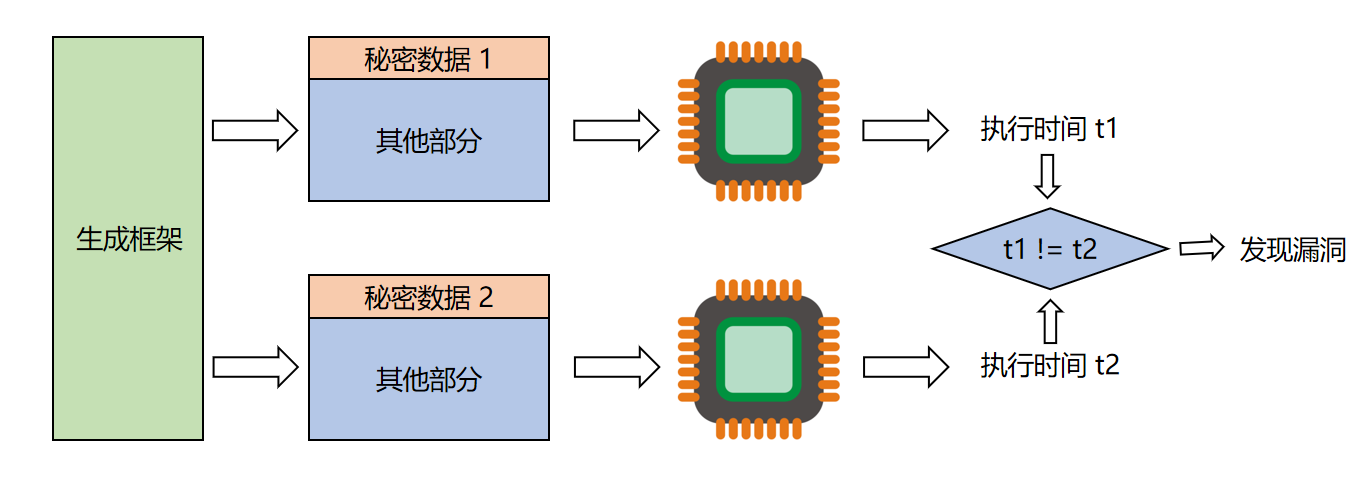
\includegraphics[width=\linewidth]{figure/paper/differential-test.png}
    \caption{差分测试流程}
    \label{paper:differential-test}
\end{figure}

\cleardoublepage
\section{测试程序生成框架的实现}

本工作由瞬态漏洞测试程序生成框架和硬件处理器插桩修改两部分组成。
其中测试程序生成框架包括 5.2 K 行 Python 和 300 行 RISCV 汇编,负责瞬态漏洞测试程序的生成、测试调用和化简;
硬件测试平台在开源 RISCV 处理器测试框架 starship\cite{starship} 的基础上进行修改,
包括 650 行 C 代码、200 行 Verilog、50 行 chisel,用于提供硬件插桩和测试功能扩展。
我们的测试程序生成框架可以支持 U、S、M 三特权级的测试程序生成,可以支持虚拟地址、物理地址的测试程序生成,
在指令生成方面支持 RISCV 的 rv64imafdc\_zicsr 基本指令扩展,可以高效生成 spectre、meltdown 等典型的瞬态漏洞测试程序。\par

\subsection{硬件插桩和功能扩展}

为了让被测试的处理器满足瞬态漏洞测试程序执行和测试的需要,我们需要对被测试的处理器硬件进行插桩和功能扩展,包括:
a)提供事件监控的软件 label 指令插桩和硬件 rob 插桩;b)提供处理器停机、结束测试程序的软件接口;
c)提供支持物理内存切换的功能的内存模块和触发物理内存切换的软件接口。\par

我们在开源的 RISCV 计算机系统评估框架 starship\cite{starship} 的基础上进行处理器硬件的修改和测试。
starship 通过继承一系列开源的 RISCV 软硬件工具,实现自动化的全栈计算机系统生成,
可以支持 rocket-chip\cite{rocket-chip}、BOOM\cite{celio2017boomv2}、CVA6\cite{cva6} 等开源 RISCV 处理器的仿真、评估、FPGA执行等。
本工作目前仅在 starship 提供的 BOOM flow 的基础上进行测试和评估,
故而下文的硬件插桩和处理器测试仅针对 BOOM 处理器而言。\par

\subsubsection{事件监控和 rob 插桩}
\textbf{label 指令:}
为了了解测试程序在处理器内部的执行情况,检查特殊事件(如瞬态窗口触发、程序执行完毕等)是否发生,
我们预留了一组 slti 指令作为特殊的 label 指令,并将它们排布在软件的合适位置作为软件插桩。
该部分指令如果被处理器执行,则意味着特殊事件发生。
所有的 label 指令表示的事件、排布的位置等如表\ref{table:label-inst}所示,
因此在生成各个代码块和将它们组织为 group 的时候需要在指定位置额外插入这些 label 指令。\par

\begin{table}[h!]
    \begin{center} 
    \caption{label指令} 
    \label{table:label-inst}  
    \resizebox{1.0\linewidth}{!}{
        \begin{tabular}{|l|l|l|l|} 
            \hline
            \textbf{label名称} & \textbf{汇编指令} & \textbf{排布位置} & \textbf{表示事件}\\
            \hline
            INFO\_VCTM\_START  &  slti zero, zero, 0  & group代码块的第一条代码  & group 开始执行            \\
            INFO\_VCTM\_END    &  slti zero, zero, 1  & group代码块的出口位置    & group 执行完毕            \\
            INFO\_DELAY\_START &  slti zero, zero, 2  & delay块的第一条代码      & 开始数据流延迟执行        \\
            INFO\_DELAY\_END   &  slti zero, zero, 3  & delay块的最后一条代码    & 瞬态窗口关闭              \\
            INFO\_TEXE\_START  &  slti zero, zero, 4  & encode块的第一条代码     & 瞬态窗口触发打开          \\
            INFO\_TEXE\_END    &  slti zero, zero, 5  & encode块的最后一条代码   &                          \\
            INFO\_LEAK\_START  &  slti zero, zero, 6  & decode块的第一条代码     & 开始进行秘密数据泄露       \\
            INFO\_LEAK\_END    &  slti zero, zero, 7  & decode块的最后一条代码   & 秘密数据泄露完毕           \\
            INFO\_INIT\_START  &  slti zero, zero, 8  & init块的第一条代码       & 开始寄存器初始化           \\
            INFO\_INIT\_END    &  slti zero, zero, 9  & init块的最后一条代码     & 寄存器初始化完毕           \\
            INFO\_BIM\_START   &  slti zero, zero, 10 & init\_bim块的第一条代码   & 开始等待 BIM 部件初始化   \\
            INFO\_BIM\_END     &  slti zero, zero, 11 & init\_bim块的最后一条代码 & BIM 部件初始化完毕        \\
            \hline
        \end{tabular}
    }
    \end{center}
\end{table}

\textbf{rob 插桩:}
我们需要对被测试处理器的 ROB 进行硬件插桩,通过监视测试程序中的 label 指令是否进入 rob 和
是否在 rob 中被提交或者回滚,判断瞬态窗口触发、瞬态窗口关闭、程序执行结束等事件是否发生,并记录这些事件发生的时间。
其中瞬态窗口触发事件的发生被用于阶段1的判断,程序执行结束的时间被用于阶段2差分测试的判断。
12 种 label 指令分别代表一类事件,根据 label 是进入 rob 还是从 rob 中提交可以分为 ENQ 和 DEQ 两种子事件,所以一共有 24 种事件。\par

rob 插桩和事件 log 记录的代码\ref{code:rob-stub}首先创建一个 taint.log 文件,
然后将监控到的事件信息 dump 到这个 log 文件中,
最后实例化两个 event\_handler 函数调用对 rob 的进入和提交进行周期性检测,
一个负责根据进入 rob 的指令类型记录 ENQ 事件发生;一个负责根据 rob 提交的指令类型记录 DEQ 事件发生。

\begin{figure}[htbp]
    \centering
    \begin{minted}{Verilog}

    initial begin
        $timeformat(-9, 0, "", 20);
        $value$plusargs("taintlog=%s", taintlog);
        event_fd = $fopen({`TOP_DIR, "/wave/", taintlog, ".taint.log"}, "w");
    end

    always @(posedge clock) begin
        if (!reset) begin
            event_handler(`DUT_ROB_ENQ_EN_0, `DUT_ROB_ENQ_INST_0, "ENQ", 0, `IS_DUT);
            event_handler(`DUT_ROB_DEQ_EN_0, `DUT_ROB_DEQ_INST_0, "DEQ", 0, `IS_DUT);
        end
    end

    \end{minted}
    \caption{rob插桩}
    \label{code:rob-stub}
\end{figure}

核心函数 event\_handler 如图\ref{code:event-handler}所示,
该函数记录 rob 检测到的事件。它接收五个参数,其中 valid 表示当前指令进入或者离开 rob,
inst 为当前指令的编码,suffix 为当前指令的子事件类别(ENQ 表示进入 rob、DEQ 表示从 rob 中提交)。
当 valid=1 时,event\_handler 函数根据 inst 和 suffix 的内容将不同的事件 log 信息保存到 taint.log 文件中,
包括事件的名称(如 TEXE\_START\_ENQ、TEXE\_END\_DEQ)和当前的处理器 cycle 数。

\begin{figure}[htbp]
    \centering
    \begin{minted}{Verilog}

    function void event_handler;
        input valid;
        input [31:0] inst;
        input string suffix;
        input int id;
        input int is_dut;

        if (valid) begin
            case (inst)
                `INFO_VCTM_START: $fwrite(event_fd, "%t, VCTM_START_%s, %d, %d\n", $time, suffix, id, is_dut);
                `INFO_VCTM_END: $fwrite(event_fd, "%t, VCTM_END_%s, %d, %d\n", $time, suffix, id, is_dut);
                ...
            endcase
        end
    endfunction
    \end{minted}
    \caption{event\_handler函数}
    \label{code:event-handler}
\end{figure}

\subsubsection{程序退出和打印}
为了在测试程序执行完毕后,结束处理器的运行,退出仿真,我们需要为处理器增加终止仿真执行的软件接口;
此外为了方便对测试程序的仿真进行调试,我们需要为处理器增加打印的软件接口。\par

这里我们为处理器扩展了一个用户态只写特权寄存器 probebuffer。该模块
内部的操作由 DPI-C 接口调用 cpp 函数实现,该函数会根据写入寄存器的值执行退出和打印操作。
为了将 probebuffer 集成到 BOOM 处理器中,我们为 BOOM 的chisel 工程提供了 BlackBox 的 verilog 接口,
并为 probebuffer 分配了 0x800 的 CSR 号。当 csrw 指令写 0x800 特权寄存器时即可调用 probebuffer 的打印和退出程序接口
(此外,probebuffer 也被用于物理内存切换,这部分内容将在下一节中介绍)。
接口的具体调用细节如下表。\par

\begin{table}[h!]
    \begin{center} 
    \caption{probebuffer 软件接口} 
    \label{table:probebuffer}  
    \resizebox{0.8\linewidth}{!}{
        \begin{tabular}{|l|l|} 
            \hline
            \textbf{输入} & \textbf{功能}\\
            \hline
            0xAF1B608E883A0000 & probebuff切换到默认工作状态 \\
            0xAF1B608E883A0001 & probebuff切换到打印整数状态 \\
            0xAF1B608E883A0002 & probebuff切换到打印字符状态 \\
            0xAF1B608E883A0003 & probebuff切换到打印地址状态 \\
            0xAF1B608E883B0000 & probebuff执行 exit 函数结束仿真进程 \\
            0xAF1B608E883C0000 & 内存单元进行物理内存切换     \\
            其他               & 根据当前工作模式调用 printf 函数输出写入数据 \\
            \hline
        \end{tabular}
    }
    \end{center}
\end{table}

\subsubsection{内存切换和管理}
为了提高 train 块训练 trigger 指令的效果,也为了提高 decode 块对 encode 块编码的解码效果,
程序执行时需要这些指令可以在相同的地址上被执行,因此需要有软硬件机制实现物理内存的指令切换,
根据设计部分的介绍可以知道,这里的物理地址切换是以 group 为单位进行的。
纯软件的物理地址切换可以考虑在执行下一个 group 之前拷贝它的 group 代码覆盖上一个 group 的代码,
这样虽然确保 group 使用同样的物理地址,但是拷贝本身的 overhead 较大,
且严重影响数据 cache 的布局,并且还要解决 icache 的同步问题,
使用效果并不理想;此外也可以通过修改页表让不同的 group 共用相同的逻辑地址,但是无法用于物理地址模式下的内存切换。
因此本工作选择将处理器的 memory 单元替换为我们实现的可切换内存单元,并暴露软件接口来进行物理内存的直接切换,
这样切换的效率最高,对 icache、dcache 的影响也最小。\par

\textbf{内存初始化配置:}
为了便于改写后的内存单元对内存进行管理和切换,生成框架在生成二进制程序的同时,还会生成一个 libconfig 格式的 config 文件,
用于指示内存单元如何进行内存初始化。config 文件的格式如图\ref{code:memory-config}所示。\par

\begin{figure}[htbp]
    \centering
    \begin{minted}{text}
        start_addr = 2147483648L;
        max_mem_size = 262144;
        memory_regions = (
            {
                type = "dut";
                start_addr = 2147483648L;
                max_len = 61440;
                init_file = "origin_common.bin";
                swap_id = 0;
            },
            ...
            {
                type = "swap";
                start_addr = 2147614720L;
                max_len = 4096;
                init_file = "text_swap_0.bin";
                swap_id = 0;
            }
        );
        swap_list = [1, 0];
    \end{minted}
    \caption{memory config}
    \label{code:memory-config}
\end{figure}

config 的 start\_addr 和 memory\_region 字段表示所需内存的起始地址和长度,内存单元在初始化时会根据这两个字段产生对应大小的内存区域。
memory\_regions 序列表示了需要被内存单元载入的内存块序列的具体信息。start\_addr 表示该内存块的起始地址,
max\_len 表示该内存块需要的内存范围
因为 memory\_region 以页为最小管理单位,所以其中 start\_addr 是页对齐的,max\_len 是 4K 的整数倍长度;
init\_file 为该内存块指令或者数据所在的 binary 文件的路径。type 表示内存块的种类,如果是 dut 表示这是一个普通的内存块,
程序的框架代码例如 trap 块、init 块、数据部分等不会被切换的内存区域就会被设置为 dut 类型。
内存单元为这个内存块分配 start\_addr-start\_addr+max\_len 的内存范围,然后读取 init\_file 中的二进制内容作为这部分内存的值。\par

如果 type 的类型是 swap,则说明这些内存区域是会被切换的,train group、victim group、decode group 因为会被切换地址范围,
所以被设置为 swap 类型,我们称这部分 memory 为 swap mem\_region。
可切换内存区域的数据不会被直接初始化到内存单元中,而是会额外分配一块处理器不可达的内存空间“可切换内存区域数组”
暂时存放这些内存区域的内容,等需要切换这块内存区域的时候,再将其替换到内存单元中。
为了便于可切换内存区域的切换和管理,config 的 memory\_region 结构还包含一个 swap\_id 字段,为每个可切换内存区域
提供了唯一的 swap 编号(这个编号对于 dut 类型的内存区域没有意义),并维护了一个 swap\_list 的数组。
当处理器执行内存切换的时候,内存单元将按照 swap\_list 中的 swap\_id 依次切换为对应的内存。\par 

在本工作的场景下,所有的可切换内存区域共用同一个物理内存地址范围,所以需要额外确保所有的可切换内存区域的 start\_addr
和 max\_len 保持一致。\par

\textbf{可切换内存单元:}
我们用 C++ 程序实现可物理内存切换的内存单元,然后用 DPI-C 接口,将它集成到处理器 Verilog 代码框架之中。
可切换内存单元提供的核心数据结构和函数接口如图\ref{code:swappable-memory}所示。\par

\begin{figure}[htbp]
    \centering
    \begin{minted}{cpp}
        void initial_mem(size_t mem_start_addr, size_t max_mem_size, std::vector<int>& schedule_list);
        void register_swap_blocks(size_t block_begin, size_t block_len, std::string &file_name, int swap_index);
        void register_normal_blocks(size_t block_begin, size_t block_len, std::string &file_name);
        void do_mem_swap();
        void write_byte(size_t addr, uint8_t data);
        uint8_t read_byte(size_t addr);
        void print_swap_mem();
    \end{minted}
    \caption{可切换内存单元}
    \label{code:swappable-memory}
\end{figure}

1.内存初始化:在处理器测试程序一开始自动执行的时候,可切换内存单元根据 memory config 文件中对内存区域的定义,进行内存初始化。
可切换内存单元的 initial\_mem 函数根据 start\_addr 和 max\_mem\_size 字段产生一个 max\_mem\_size/4K 大小的指针数组 mem\_block\_array,
每个表项用于指向对应的页数据。每一个 dut mem\_region 表项通过 register\_normal\_blocks 生成一个大小为 max\_len、载入对应文件二进制数据的连续内存,
然后 mem\_block\_array 对应的页表项指向 normal mem\_region 的页起始地址,用这样的方法将内存单元的一个 dut 内存区域载入对应的指令和数据。
每一个 swap mem\_region 表项通过 register\_swap\_blocks 函数生成一个生成一个大小为 max\_len、载入对应文件二进制数据的连续内存,
它的 swap\_id 和 mem\_region 被保存到 swap\_block\_map 当中,而 swap\_list 的数据被保存到 swap\_schedule 当中。
初始完成后的可切换内存单元数据布局如图\ref{paper:swap-mem-init}所示。\par

\begin{figure}[!h]
    \centering
    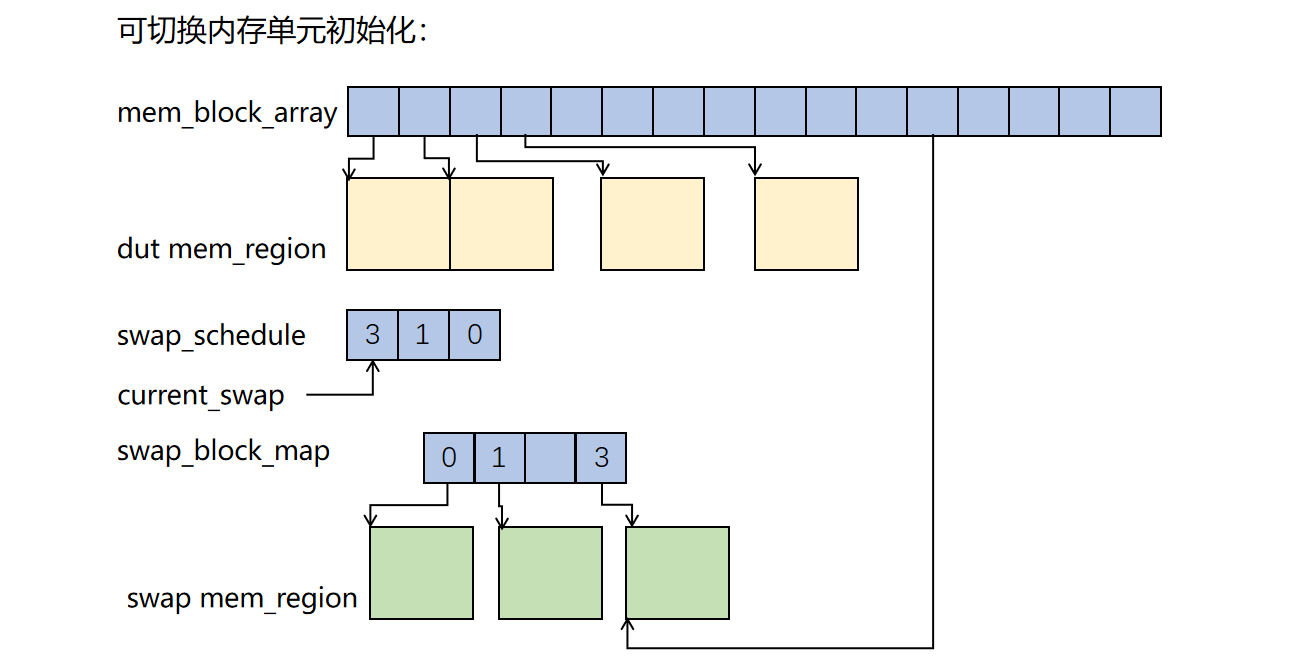
\includegraphics[width=\linewidth]{figure/paper/swap-mem-init.png}
    \caption{可切换内存单元初始化}
    \label{paper:swap-mem-init}
\end{figure}

2.内存读写操作:内存单元的读操作通过 DPI-C 接口调用可切换内存单元的 read\_byte 函数执行。该函数传入物理地址返回对应的字节。
首先根据传入的物理地址 addr 计算对应的页号和页内偏移,然后根据页号查找 mem\_block\_array 对应表现的数组指针(如图\ref{paper:swap-mem-addr}步骤1),如果指针为空,
则说明内存没有被分配,分配一个全 0xff 的内存,然后读取数据;不然根据指针找到对应的 mem\_region 页,
然后根据页内偏移即可定位待操作的字节(如图\ref{paper:swap-mem-addr}步骤2),
然后读取该字节的数据即可。写操作利用 DPI-C 接口调用可切换内存单元的 write\_byte 函数执行,
它采用和 read\_byte 一样的方式找到对应的字节,然后进行数据写入。\par

\begin{figure}[!h]
    \centering
    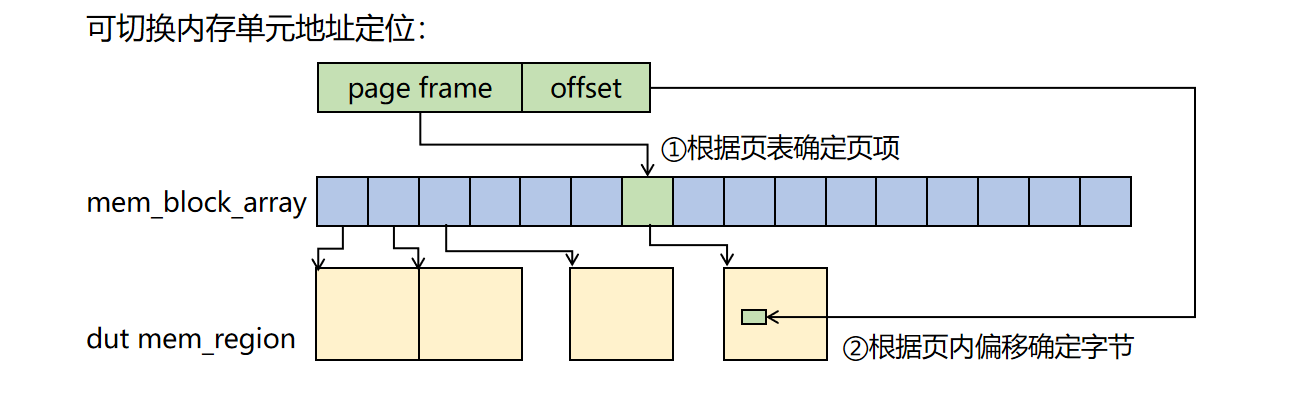
\includegraphics[width=\linewidth]{figure/paper/swap-mem-addr.png}
    \caption{可切换内存单元地址定位}
    \label{paper:swap-mem-addr}
\end{figure}

3. 内存切换操作:内存单元的切换操作通过可切换内存单元的 do\_mem\_swap 函数执行。current\_swap 记录了当前切换的 swap mem\_region 在
swap\_schedule 的序号,然后将 current\_swap 递增,得到下一个需要切换的 swap mem\_region 的 swap\_id,然后通过查询 swap\_block\_map 
找到对应的 swap mem\_region。最后将 mem\_block\_array 对应地址范围的页表项指针指向该 mem\_region 的页起始地址即可。
整个 swap\_schedule 的切换流程如图\ref{paper:swap-mem-swap}所示。\par

\begin{figure}[!h]
    \centering
    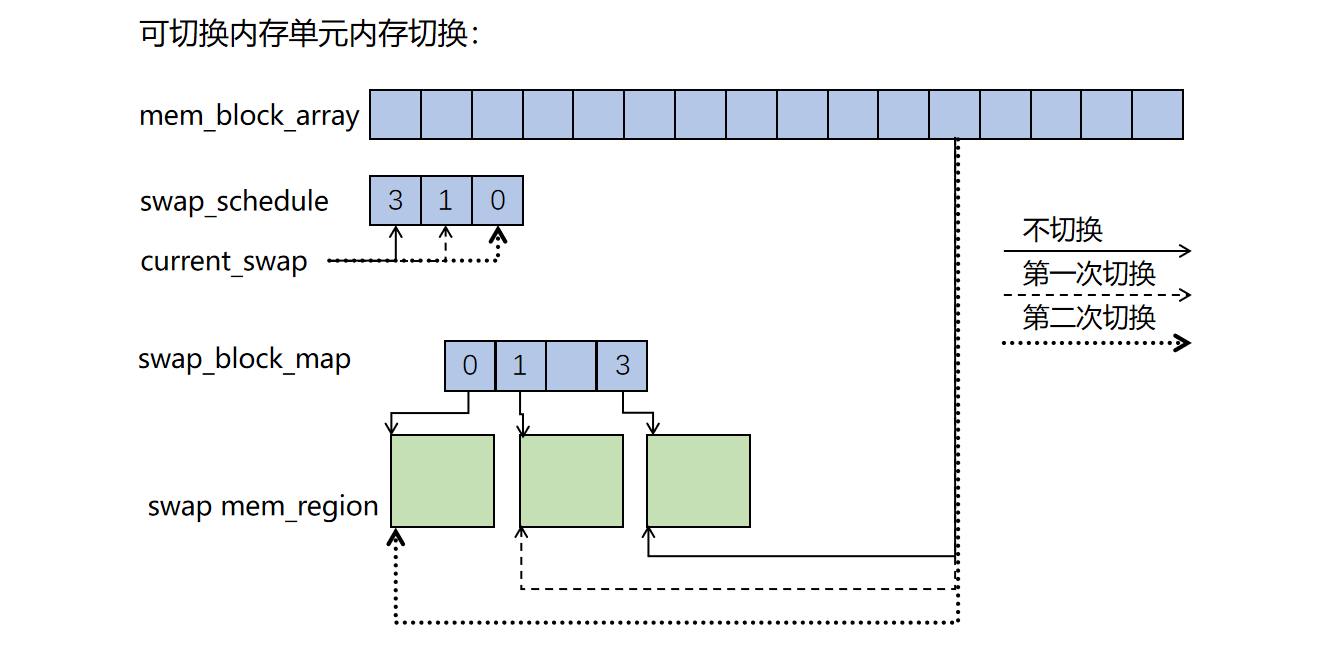
\includegraphics[width=\linewidth]{figure/paper/swap-mem-swap.png}
    \caption{可切换内存单元内存切换}
    \label{paper:swap-mem-swap}
\end{figure}

因为所有 swap mem\_region 共用物理地址,所以该操作也同时移除了物理内存中的上一个 swap mem\_region。
如果 swap\_schedule 的所有 swap mem\_region 都被切换使用,程序异常终止,但是生成的测试程序保证处理器在最后一个 swap mem\_region 终止,
故而可以规避这一问题。\par

为了测试程序的软件可以主动调用内存切换功能,来进行 train group、victim group、decode group 之间的切换,因此
可切换内存单元需要为软件暴露编程接口。我们将这个接口集成到 probebuffer 当中,如果 probebuffer 寄存器写入 0xAF1B608E883B0000
即可执行内存切换。

\textbf{生成框架协同:}
参照图\ref{paper:group-switch-all},测试程序的执行流程是先执行初始部分代码,然后用内存切换机制依次执行 train group 序列、
victim group 序列、decode group 序列,然后执行 exit 块的代码退出。为了简化 group 之间的跳转流程,生成框架将 exit 块建模为
 exit group,作为所有共用地址的 swap mem\_region 的最后一个,这样当测试程序依次切换 swap\_schedule 的 swap mem\_region 时就可以
在最后一个 swap mem\_region 执行 exit 块的代码结束测试。这也确保了测试程序在 swap\_schedule 的 swap mem\_region 耗尽之前可以结束程序。\par

测试程序包括框架代码和各个 group 各自的代码,当测试程序进行二进制生成的时候,首先生成一个 elf 程序,然后转换为对应的二进制。
但是因为各个 group 共用同一个物理地址,这导致单次生成的 elf 无法直接包含所有 group 的二进制内容。因此生成框架每次只用一个 group 的
汇编代码和框架代码组合生成一个二进制文件,然后根据程序的符号表,将二进制文件切割为框架代码的二进制部分(dut mem\_region)和 group 代码的
二进制部分(swap mem\_region)。最后所有的 dut mem\_region 和swap mem\_region 按照 config 指定格式生成 config 文件即可。\par

最后为了方便测试程序在执行的时候进行内存切换,生成框架将内存切换的代码(将 0xAF1B608E883B0000 写入 0x800 寄存器)放置在 trap 块,然后
将 return 块、trans 块、encode 块、nop\_return 块等退出 group 的出口指令由原来的跳转指令修改为 ebreak 指令。
这样无论是因为触发异常退出 group,还是从控制流出口正常退出都会最终在 trap 块内部执行内存切换的代码,完成内存切换。
trap 块末尾将返回地址修改为 group 的入口地址退出异常处理程序,即可开始执行下一个 group 的代码。
内存切换和执行流程如图\ref{paper:execute-flow}所示。\par

\begin{figure}[!h]
    \centering
    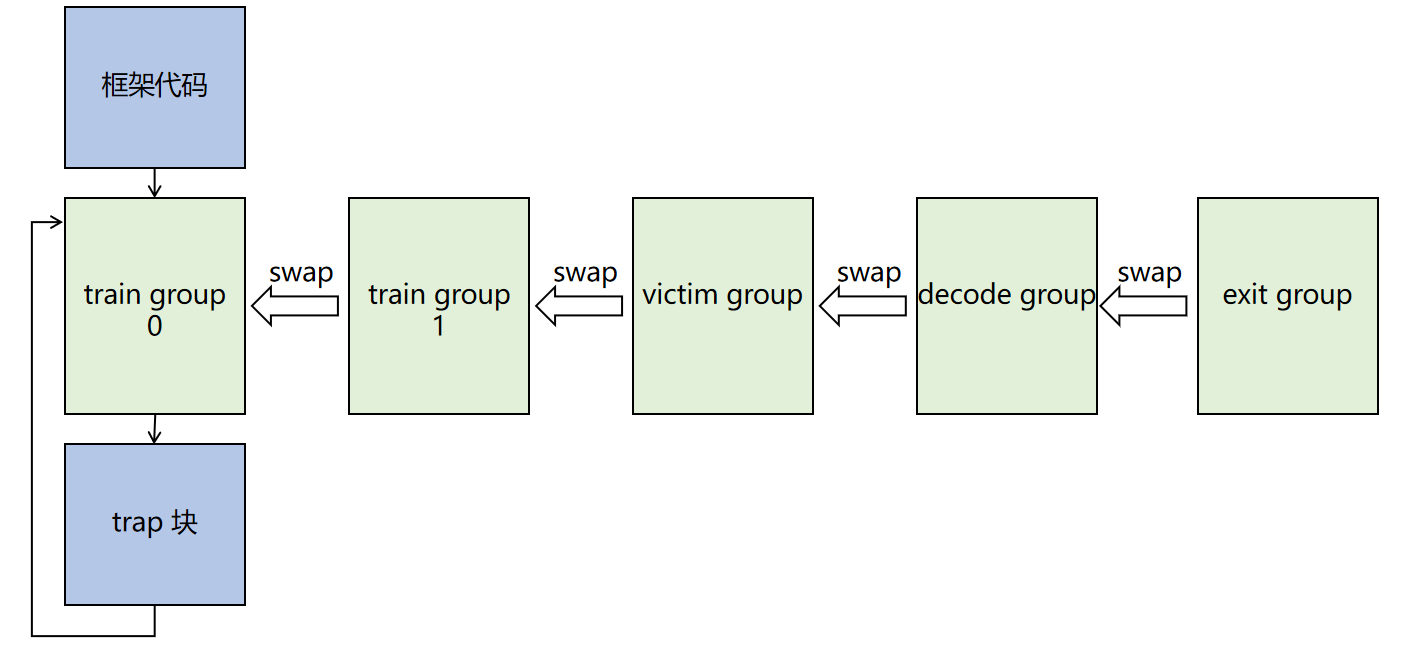
\includegraphics[width=\linewidth]{figure/paper/execute-flow.png}
    \caption{程序执行和内存切换流程}
    \label{paper:execute-flow}
\end{figure}

\subsection{框架组件生成}

为了生成可以执行的程序,生成框架不但要生成 trigger 块、train 块等用于触发瞬态窗口和侧信道泄露秘密数据的 poc 代码,
还需要额外生成一些框架代码,用于支持 poc 代码的执行和生效。本章节将对这些框架相关的代码部分、数据部分、其他机制进行罗列和详细介绍。\par

\subsubsection{框架代码块和框架数据块}
本章节将对框架相关的代码部分、数据部分进行罗列和详细介绍。

\textbf{全局初始化块(init 块):}
init 块用于对所有 GPR、FPR、CSR、PC 和特权级进行初始化。为了对寄存器,特别是特权寄存器继续 field 粒度的属性设置,
本工作实现了 snapshot 模块作为子模块。该模块会读入一个 reg\_init.hjson,这个文件记录了通用寄存器 GPR、浮点寄存器 FPR、
M态和S态的基本特权寄存器 field 粒度的属性值,然后拼接 CSR 的各个 field 得到 CSR 的初始值,并生成寄存器初始化的汇编代码。
该汇编代码将所有 CSR、FPR、GPR 的初始化值存储为一个 64 位数据的数组,然后依次读取数据的值来初始化 CSR、FPR、GPR 的值。
生成框架的 InitManager 负责修改 reg\_init.hjson 各个字段的值,为每个特权寄存器提供满足测试程序要求的值,
并调用 snapshot 模块得到对应的初始化程序。例如 mtvec 和 stvec 需要设置为 trap 块的入口地址,satp 设置为页表基地址,
mstatus 的 pmie 设置为程序执行所需要的特权级,mepc 设置为后续程序执行的入口地址,然后在 init 块末尾执行 mret,
进入后续测试程序的入口,并自动设置程序执行时的特权级。\par

\textbf{BIM 初始化块(init\_bim 块):}
init\_bim 块用于等待处理器的 BIM 分支预测部件进行初始化。BOOM 等处理器使用 BIM 前端部件进行分支预测,BIM 是一个拥有众多表项
的庞大 sram(例如 BOOM 的 BIM 是 2048 项的),处理器在启动的时候会将 BIM 的表项依次进行初始化为初始状态。
为了使瞬态执行漏洞测试程序在攻击时,处理器的 BIM 组件已经进入工作状态,从而使测试程序的执行环境和真实环境一致,
生成框架在这里插入了一段延时的循环,用于等待 BIM 部件各个表项初始化完毕。当 init 块完成寄存器初始化之后,首先进入
init\_bim 块等待 BIM 的初始化,当 init\_bim 块执行完毕后执行 ebreak 指令进入 trap 块开始执行内存切换。\par

\textbf{异常块(trap块):}
trap 块用于 group 的退出和物理内存的切换。当一个 group 执行完毕后就会进入 trap 块,然后 trap 块指令将操作数 0xAF1B608E883C0000
写入 probebuffer 寄存器进行内存切换,之后执行 fence 指令刷新 pipeline、icache 和 tlb 的指令缓存,完整指令内存在处理器内部的同步。
之后将返回地址设置为 group 的入口地址(所有 group 入口地址保持统一)后返回下一个 group 入口进行执行。为了可以监控 group 开始执行和
执行结束两个事件的发生,生成框架在 trap 的入口插入一条 INFO\_VCTM\_END 表示 group 执行结束,在 sret/mret 前插入一条 INFO\_VCTM\_START 表示 group 开始执行。
因为 trap 块在 M 模式下和 S 模式下需要不同的页表权限;而且 trap 在做内存访问的时候,M 模式下直接使用 label 对应的物理地址,
但是 S 模式下需要将 label 加上常数偏移量,得到 S 模式专用的 FFF 开头的地址才可以开始内存访问。
因此这里实际上会生成 mtrap 块和 strap 块两个代码块,
init 块会将 mtvec 设置为 mtrap 的入口,stvec 设置为 strap 的入口。\par

\textbf{退出块(exit 块):}
exit 块作为最后一个 swap mem\_region、exit group 唯一的块,被用于测试程序的退出。
该模块将 0xAF1B608E883CB0000 写入 probebuffer 寄存器,结束程序。\par

\textbf{秘密数据块(secret 块):}
secret 块用于存放秘密数据,是瞬态漏洞执行程序泄漏的目标。secret 被初始化为一些魔数,并且生成框架确保测试程序只会在
 access\_secret 块和 secret\_migrate 块中访问 secret 数据,确保程序不在其他位置显式或者瞬态访问 secret 数据。
当执行差分测试时,变体测试程序会将 secret 部分替换为全 0,然后进行后续的差分测试。\par

\textbf{信道数据块(channel 块):}
channel 块是预留给 cache 微架构状态编码的内存区域。channel 由 256 个 64 字节组成,每 64 字节是一个 cacheline 的长度,
可以使用 access\_secret 得到的一字节 secret 作为索引访问 channel,从而实现将 secret 编码到 cache 进行数据泄露的目的。\par

\textbf{随机数据块(random\_data 块):}
random\_data 块是两页随机数据。train 块、encode 块、trigger 块等代码块有时会执行随机内存访问,则生成框架可以让这些内存
读写指令访问 random\_data 块的数据,这样既不会破坏其他重要数据区域,又可以为数据流引入新的随机数,增加执行流的复杂程度和覆盖率。\par

\textbf{无用数据块(dummy\_data 块):}
dummy\_data 块内部的数据值没有意义,该块由四页内存空间组成,secret\_migrate 块通过访问 dummy\_data 块来调整 cache 的状态。\par

\textbf{访问异常数据块(access\_fault\_data 块):}
access\_fault\_data 块提供了一页被 pmpaddr、pmpcfg 设置为禁止访问的数据页。生成框架如果想要产生一个 load\_access\_fault 异常或者
store\_access\_fault 异常就可以让 load、store 指令访问这个页,然后触发异常。\par

\textbf{页错误数据块(page\_fault\_data 块):}
page\_fault\_data 块提供了一页被页表设置为禁止访问的数据页。生成框架如果想要产生一个 load\_page\_fault 异常或者
store\_page\_fault 异常就可以让 load、store 指令访问这个页,然后触发异常。\par

\textbf{堆栈块(stack 块):}
stack 块被用于作为程序的堆栈部分,该部分暂时未被启用。如果后续生成框架需要产生了类似 C 语言那样的函数调用、递归调用、局部变量等场景,可以考虑启用该块作为堆栈。\par

\textbf{框架数据块(data\_frame 块):}
data\_frame 块用于存放框架部分代码的数据,比如 exit 块要访问的数据。\par

\textbf{训练数据块(data\_train 块):}
data\_train 块用于存放所有 train group 需要使用的数据,例如每个 train group 的 load\_init\_train 块的寄存器初始化数据。
理论上让每个 group 的数据跟着指令一起做 swap 是最简洁,但是因为 dcache 的数据无法被刷新,这就导致如果数据物理内存发生切换,
并没有高效的方法让 dcache 中的数据进行同步,因此只能让 group 的数据分别使用不相交的地址空间。\par

\textbf{受害数据块(data\_victim 块):}
data\_victim 块用于存放 victim group 需要使用的数据,例如 victim group 的 load\_init 块的寄存器初始化数据。\par

\textbf{解码数据块(data\_decode 块):}
data\_decode 块用于存放 decode group 需要使用的数据,例如 decode group 的 load\_init 块的寄存器初始化数据。\par

\subsubsection{地址分布}

本章节我们介绍生成框架的地址分布和地址管理。生成框架下处理器内存的物理地址范围是 0x80000000-0x80040000,总计 64 KB 的内存范围。
因为生成框架生成的代码可能同时包含了 M 态、S 态、U 态执行的代码,对于不同特权态下运行的代码需要生成不同的逻辑地址。
对于 M 态的代码,其逻辑地址和物理地址保持一致,地址格式为 0x800xxxxx。对于 U 态的代码则在物理地址的基础上加一个常数偏移量作为逻辑地址,
地址格式为 0x000xxxxxxx。对于 S 态的代码因为页表项 U 位的设置无法和 U 态的代码共用一份逻辑地址,因此加上另一个常数偏移量,地址格式为
0xfffxxxxx。\par

测试程序生成的 section,每个 section 的虚拟地址范围、物理地址范围和权限,每个 section 的代码块、
数据块组成参见表\ref{table:section-dist}、\ref{table:group-dist}:

\begin{table}[h!]
    \begin{center} 
    \caption{section地址排布} 
    \label{table:section-dist}  
    \resizebox{1.0\linewidth}{!}{
        \begin{tabular}{|l|l|l|l|l|l|l|} 
            \hline
            \textbf{section名称} & \textbf{包含的block} & \textbf{M 模式基址} & \textbf{S 模式基址} & \textbf{U 模式基址} & \textbf{长度} & \textbf{权限} \\
            \hline
            .init       &   init 块     &   0x80000000  &   \textasciitilde &   \textasciitilde &   1K  &   物理模式     \\ 
            .pagetable  &   pgtlb块     &   0x80001000  &   \textasciitilde &   \textasciitilde &   3K  &   物理模式     \\
            .secret     &   secret块    &   0x80004000  &   0xfff04000      &   0x00004000      &   1K  &   URW             \\ 
            .channel    &   channel块   &   0x80005000  &   0xfff05000      &   0x00005000      &   4K  &   URW             \\ 
            .mtrap      &   mtrap块     &   0x80009000  &   \textasciitilde &   \textasciitilde &   1K  &   物理模式     \\
            .strap      &   strap块     &   0x8000a000  &   0xfff0a000      &   0x0000a000      &   1K  &   RWX             \\
            .text\_frame &   init\_bim块  &   0x8000b000  &   0xfff0b000      &   0x0000b000      &   1K  &   URX              \\
            .random\_data&   random\_data块&  0x8000c000  &   0xfff0c000      &   0x0000c000      &   2K  &   URW              \\
            .data\_frame &   data\_frame块&   0x8000e000  &   0xfff0e000      &   0x0000e000      &   1K  &   URW              \\
            .data\_frame &   data\_victim块&  0x8000f000  &   0xfff0f000      &   0x0000f000      &   1K  &   URW              \\
            .data\_frame &   data\_decode块&  0x80010000  &   0xfff10000      &   0x00010000      &   1K  &   URW              \\
            .data\_frame &   data\_train块&   0x80011000  &   0xfff11000      &   0x00011000      &   1K  &   URW              \\
            .text\_swap  &   见表\ref{table:group-dist}  &   0x80020000  &   0xfff20000      &   0x00020000      &   1K  &   URX              \\
            .dummy\_data &   dummy\_data块&   0x80038000  &   0xfff38000      &   0x00038000      &   4K  &   URW              \\
            .access\_fault\_data  &   access\_fault\_data块 &   0x8003c000  &   0xfff3c000  &   0x0003c000  &   1K  &   不可访问 \\
            .page\_fault\_data    &   page\_fault\_data块   &   0x8003d000  &   0xfff3d000  &   0x0003d000  &   1K  &   物理模式 \\
            .stack      &   stack块     &   0x8003e000  &   0xfff3e000  &   0x0003e000  &   2K  &  RW \\
            \hline
        \end{tabular}
    }
    \end{center}
\end{table}

\begin{table}[h!]
    \begin{center} 
    \caption{group的.swap\_text包含的代码块} 
    \label{table:group-dist}  
    \resizebox{0.9\linewidth}{!}{
        \begin{tabular}{|l|l|} 
            \hline
            \textbf{group名称} & \textbf{包含的block} \\
            \hline
            train group  & load\_init\_train 块,nop 块,train 块,nop\_return 块,return 块 \\
            victim group & load\_init 块,nop 块,secret\_migrate 块,delay 块,trigger 块,\\
                         & access\_secret 块,encode 块,return 块 \\
            decode group & load\_init 块,nop 块,delay 块,replace 块,decode 块,return 块 \\
            exit group   & exit 块 \\
            \hline
        \end{tabular}
    }
    \end{center}
\end{table}

参照表中对于各个部分的地址分配和权限分配, 生成框架的 PageTableManager 生成页表的数据段,
包括虚拟地址和物理地址的映射,以及访问权限的设置。
其中对于用户态的代码和数据页都需要一个额外的内核态的页表项进行映射,
确保当程序在 S 模式执行时仍然可以顺利执行。生成框架的 LinkManager 生成对应的链接脚本,将各个段链接起来。\par

\subsection{策略生成}

为了使得 train group、victim group、decode group 中的各个代码块有较好的指令覆盖率和训练效果,
生成框架对每一个代码块都制定了有针对性的生成策略。本章节将对每个代码块的生成策略进行详细介绍。
为了可以对指令的字段和操作数进行约束求解,本工作扩展开源的 RISCV 指令生成工具razzle\cite{razzle}作为基础指令生成器。

\subsubsection{瞬态窗口触发部分}

瞬态触发相关的重要代码块包括 train group 的训练块(train 块)和trigger group 的触发块(trigger 块)、
延迟块(delay 块)。我们依次对每个块的生成策略进行介绍。\par

\textbf{延迟块(delay块):}\par
delay 块的目的在于让后续的 trigger 块延迟获得操作数结果,迫使 trigger 块预测执行。为了防止延迟块的指令影响前端部件
和内存部件的微架构状态,delay 块主要采用整数运算指令、乘除法扩展指令、单精度浮点指令和双精度浮点指令进行运算。
为了可以让指令的计算尽可能的耗时,delay 块应该尽可能多的采用多周期指令,且指令序列之间应该有较强的数据流依赖,
以确保指令的计算开销可以不断累加起来。\par

为了检验哪些类型的指令组合可以产生较长时间的延迟,进而打开足够大的瞬态窗口,我们进行了如下实验:该实验用浮点指令组合和整型指令组合
充当 delay 块,相邻指令之间有数据依赖,用分支预测指令作为 trigger 块,在瞬态窗口中填充 INFO\_TEXT\_START 指令。然后我们执行该测试程序,检查 rob 插桩
监测到的 INFO\_TEXT\_START 指令条目,以此来估计瞬态窗口的大小。测试结果如表\ref{table:float-seq}、\ref{table:int-seq}所示。\par

观察表\ref{table:float-seq}可以看到,一条浮点指令触发的瞬态窗口长度为 8 条指令,一条浮点指令触发的瞬态窗口长度在 14-22 条指令之间,
三条浮点以上指令触发的瞬态窗口长度在 17-24 条指令之间,最大不超过 24 条指令。故而只要有 3-5 条指令基本上就可以有 22-24 条指令的瞬态窗口,
继续增加浮点指令的长度并不能显著提高。故而浮点指令数目在 3-5,即可打开 20-24 大小的瞬态窗口,继续增长指令序列没有意义。\par

\begin{table}[h!]
    \begin{center} 
    \caption{浮点指令组合} 
    \label{table:float-seq}  
    \resizebox{1.0\linewidth}{!}{
        \begin{tabular}{|l|l|l|l|l|l|} 
            \hline
            \textbf{指令类型} & \textbf{扩展类型} & \textbf{窗口宽度} & \textbf{指令类型} & \textbf{扩展类型} & \textbf{窗口宽度}\\
            \hline
            cvt                & 1 F/D & 8  & nmadd fsgnjx fcvt                             & 3 F/D & 21 \\
            nmadd fcvt         & 2 F/D & 14 & nmadd fcvt   fcvt                             & 3 F/D & 21 \\
            madd  fcvt         & 2 F/D & 14 & sgnjx fmin   fmadd  fcvt                      & 4 F/D & 24 \\
            cvt   fcvt         & 2 F/D & 15 & sgnjx fsqrt  fsqrt  fsqrt  fcvt               & 5 F/D & 21 \\
            sub   fcvt         & 2 F/D & 22 & add   fmax   fdiv   fmax   fcvt               & 5 F/D & 24 \\
            sgnjn fmadd  fcvt  & 3 F/D & 17 & div   fdiv   fdiv   fidv   fidv   fdiv   fcvt & 7 F/D & 24 \\
            madd  fmadd  fcvt  & 3 F/D & 20 &                                               &       &    \\
            \hline
        \end{tabular}
    }
    \end{center}
\end{table}

观察表\ref{table:int-seq}可以看到,任何指令序列都可以打开大小为 3 的瞬态窗口,这说明 branch 预测本身就会导致 3 个周期的瞬态窗口。
3 条整形指令无法进一步扩大瞬态窗口,1 条乘除法指令和 2 条立即数指令配合可以打开 10-12 大小的瞬态窗口,
2 条乘除法指令和 1 条立即数指令配合可以打开 20-24 大小的瞬态窗口,最大窗口不超过 24 条指令。
可以看到只有 M 扩展的指令可以扩大瞬态窗口,其中 div/rem 指令的效果略好于 mul 指令,乘法指令在 3-5 条大概率可以打开最大瞬态窗口。\par

\begin{table}[h!]
    \begin{center} 
    \caption{整数指令组合} 
    \label{table:int-seq}  
    \resizebox{0.9\linewidth}{!}{
        \begin{tabular}{|l|l|l|l|l|l|} 
            \hline
            \textbf{指令类型} & \textbf{扩展类型} & \textbf{窗口宽度} & \textbf{指令类型} & \textbf{扩展类型} & \textbf{窗口宽度}\\
            \hline
                and    and    and           & 3 I       &  3  & mulu   remu   sltu          & 1 I + 2 M &  20 \\
                srlw   mulhsu addiw         & 2 I + 1 M &  10 & div    srli   sub           & 2 I + 1 I &  21 \\
                mulhsu add    divu          & 2 I + 1 M &  12 & divw   addiw  div           & 1 I + 2 M &  24 \\
                sub    divw   add           & 2 I + 1 M &  14 & mulw   sll    slliw   srli  & 3 I + 1 M &  12 \\
            \hline
        \end{tabular}
    }
    \end{center}
\end{table}

最终我们得到结论:序列长度为 3-5 的 M 型指令和 F 型指令混合序列即可以打开大小在 18-24 之间的瞬态窗口。这里预留了两个参数,
一个是指令序列的长度,一个是浮点指令的占比,这两个参数可以由外部的配置生成器来产生。\par

延迟块的生成步骤如下:
\begin{enumerate}
    \item 生成寄存器依赖序列:在 delay 块生成时,根据超参数指令序列长度和浮点指令占比,随机产生一个数据流依赖序列,然后开始根据这个依赖序列依次进行指令生成。
考虑到 trigger 块的 trigger 指令基本都是整型指令,因此最后得到的计算结果需要在通用寄存器中,
故而数据流依赖序列的最后一个寄存器为一个随机的通用寄存器。\par

    \item 生成指令序列:之后根据依赖序列依次构造指令。
如果源寄存器和目的寄存器都是浮点寄存器则生成浮点指令,如果都是整数寄存器则生成 M 扩展指令,
如果一个是浮点寄存器,一个是通用寄存器,则生成整数、浮点数转换指令,由此得到指令序列。\par

    \item 事件管理:生成框架对 delay 块做适当调整,为了监控 delay 操作的开始和瞬态窗口的关闭,在 delay 块的开始插入 INFO\_DELAY\_START 指令,在
delay 块的末尾插入 INFO\_DELAY\_END 指令。\par

    \item 操作数调整:因为浮点操作的计算结果很容易是全 0 和全 F 的极端值,
这种值在特殊情况下会导致后续 trigger 指令的指令约束永远无法满足。因此这里再随机产生一条指令,让结果寄存器和一个随机数做加法,
让计算结果几乎以 100\% 的不为全 0 和全 F。至此 delay 块生成完毕。\par
\end{enumerate}

\textbf{触发块(trigger 块):}\par
触发块用于产生触发瞬态窗口的代码,主要是利用这部分代码的预测执行错误来产生错误的执行流。生成框架将瞬态窗口执行的 trigger 指令
分为了 22 类,囊括了 rv64imafdc 的所有指令和 zicsr 扩展的部分指令。
22 种 trigger 指令的类别、含义、需要满足的约束如表\ref{table:trigger-gen}所示。
trigger 指令的种类被作为该块的外部配置被配置生成单元管理。trigger 块的生成包括如下两个部分:\par

\begin{table}[h!]
    \begin{center} 
    \caption{触发块指令生成} 
    \label{table:trigger-gen}  
    \resizebox{1.0\linewidth}{!}{
        \begin{tabular}{|l|l|l|} 
            \hline
            \textbf{指令类型} & \textbf{类别解释} & \textbf{操作数约束}\\
            \hline
            LOAD\_MISALIGN      &   触发load\_misalign 异常           & 内存访问地址不对齐                                         \\
            LOAD\_ACCESS\_FAULT &   触发load\_access\_fault 异常      & 地址对齐且落在 access\_fault\_data 块               \\
            LOAD\_PAGE\_FAULT   &   触发load\_page\_fault 异常        & 内存对齐且落在 page\_fault\_data 块                 \\
            STORE\_MISALIGN     &   触发store\_misalign 异常     & 内存访问地址不对齐                                         \\ 
            STORE\_ACCESS\_FAULT&   触发store\_access\_fault 异常& 地址对齐且落在 access\_fault\_data 块               \\
            STORE\_PAGE\_FAULT  &   触发store\_page\_fault 异常  & 地址对齐且落在 page\_fault\_data 块                 \\
            AMO\_MISALIGN       &   触发amo\_misalign 异常       & 内存访问地址不对齐                                         \\ 
            AMO\_ACCESS\_FAULT  &   触发amo\_access\_fault 异常  & 地址对齐且落在 access\_fault\_data 块               \\
            AMO\_PAGE\_FAULT    &   触发amo\_page\_fault 异常    & 地址对齐且落在 page\_fault\_data 块                 \\
            EBREAK              &   ebreak指令触发ebreak异常                  & \textasciitilde                                             \\
            ILLEGAL             &   illegal指令触发illegal异常                & \textasciitilde                                             \\
            ECALL               &   ecall指令触发ecall异常                    & \textasciitilde                                             \\
            V4                  &   store指令与load指令地址冲突                &  操作数a0为access\_secret的访问地址                      \\
            BRANCH              &   分支预测指令,如beq、bne等                 &  控制流转移到 return 块    \\
            JALR                &   jalr指令                                 &  跳转目标为 return 块                                        \\
            RETURN              &   return指令                               &  跳转目标为 return 块                                        \\
            JMP                 &   jal指令                                  &  跳转目标为 return 块                                        \\
            INT                 &   整数运算指令和对应的压缩指令      & \textasciitilde                                             \\
            FLOAT               &   浮点运算指令和对应的压缩指令    & \textasciitilde                                             \\
            LOAD                &   内存载入指令且不触发异常          & 地址对齐且落在 random\_data 块                 \\ 
            STORE               &   内存存储指令且不触发异常          & 地址对齐且落在 random\_data 块                    \\ 
            AMO                 &   原子指令且不触发异常                       & 地址对齐且落在 random\_data 块                    \\ 
            \hline
        \end{tabular}
    }
    \end{center}
\end{table}

\begin{enumerate}
    \item 构造数据流延迟依赖:为了让 trigger 指令的操作数被延迟获得,生成框架为 trigger 指令的源寄存器和 delay 块的计算结果 delay\_reg 的值产生数据依赖。
    因为 trigger 的指令操作数需要满足特殊的条件约束,例如访存指令只能访问给定的地址区域,跳转指令只能跳入 return 块等,因此需要对
    trigger 指令操作数的值进行约束。\par
    \item 操作数约束调整:因为操作数依赖的 delay\_reg 是随机产生的,所以生成框架使用寄存器 a0 存储满足约束的调整值,
    当 a0 和 delay\_reg 相加后即可得到满足约束条件的操作数值。为了防止 a0 寄存器的值被中途改写,delay 块不允许使用 a0 寄存器参与计算。\par
\end{enumerate}

可以参看图\ref{code:trigger-example}的代码样例,这里 t0 寄存器是 delay 块的计算结果。a0 寄存器的参数值是 0,
在执行 add 指令之后 a0 寄存器的值等于 t0 寄存器,且 a0 寄存器的值依赖于 t0 寄存器。之后执行 beq 指令,因为 t0、a0 都依赖于
delay 块,所以 branch 指令会被延迟提交开始分支预测;因为 a0 参数调整使得 t0 等于 a0,所以可以跳转到 return\_block\_entry,
进入 return 块。\par

\begin{figure}[htbp]
    \centering
    \begin{minted}{c}
        add a0, t0, a0
        beq a0, t0, return_block_entry
    \end{minted}
    \caption{trigger样例}
    \label{code:trigger-example}
\end{figure}

\textbf{训练块(train 块):}\par
训练块用于对瞬态窗口进行训练,为了覆盖尽可能多的指令种类,train 块的训练指令被细分为 12 类,囊括 rv64imafdc 的所有指令和 zicsr 的部分指令。
所有 12 类指令的类别、含义、满足的约束如表\ref{table:train-gen}所示。其中内存指定范围指的是 random\_data 块、page\_fault\_data 块和 
access\_fault\_data 块。\par

\begin{table}[h!]
    \begin{center} 
    \caption{训练块指令生成} 
    \label{table:train-gen}  
    \resizebox{1.0\linewidth}{!}{
        \begin{tabular}{|l|l|l|} 
            \hline
            \textbf{指令类型} & \textbf{类别解释} & \textbf{操作数约束}\\
            \hline
            TAKEN               &   分支预测指令且发生跳转                     &  跳转目标为 return 块或者 nop\_return 块,发生跳转              \\
            NOT\_TAKEN          &   分支预测指令且不发生跳转                   &  跳转目标为 return 块或者 nop\_return 块,不发生跳转            \\
            JALR                &   jalr指令                                 &  跳转目标为 return 块或者 nop\_return 块                                        \\ 
            CALL                &   call指令                                 &  跳转目标为 return 块或者 nop\_return 块                                        \\
            RETURN              &   return指令                               &  跳转目标为 return 块或者 nop\_return 块                                        \\
            JMP                 &   jal指令                                  &  跳转目标为 return 块或者 nop\_return 块                                        \\
            INT                 &   整数运算指令和对应的压缩指令      & \textasciitilde                                             \\
            FLOAT               &   浮点运算指令和对应的压缩指令    & \textasciitilde                                             \\
            LOAD                &   内存载入指令,且不触发异常          & 访问内存地址落在指定范围内\\
            STORE               &   内存存储指令,且不触发异常          & 访问内存地址落在指定范围内\\
            AMO                 &   原子指令且不触发异常                       & 访问内存地址落在指定范围内\\
            SYSTEM              &   系统指令               & \textasciitilde                                             \\ 
            \hline
        \end{tabular}
    }
    \end{center}
\end{table}

train 块根据是否和 trigger 对齐、是否是单条指令共有三种变体。变体一为指令对齐且单条指令,该类型随机生成某一类指令,然后将该指令和 trigger 指令对齐,
寄存器的值由 load\_init\_train 提供,确保操作数满足指令约束。变体二为指令不对齐且单条指令,该类型随机生成某一类指令,
但是排布位置在 trigger 指令地址的基础上随机偏移一段距离。变体三为指令多条指令,此时讨论指令对齐没有意义,
该变体使用 arbitrary 块生成训练。\par

\textbf{随机块(arbitrary 块):}\par
为了提高测试程序的指令组合的覆盖率,生成框架需要一些纯随机的指令块进行测试。其生成过程包括如下两个步骤:
\begin{enumerate}
    \item 随机指令生成:生成框架提供了五类随机指令生成函数(函数功能参见表\ref{table:random-gen}),用于生成整型、浮点、内存访问、原子操作、系统调用指令。
为了防止修改特权寄存器导致测试程序无法正常工作,这里不生成 CSR 读写指令。\par
    \item 指令块生成和组合:arbitrary 块参考 razzle 的随机代码生成方式,首先随机生成若干个基本块,每个基本块随机用上述五个函数生成若干条指令,
    然后将这些基本块之间用 branch 和 jmp 等控制流指令连接起来,确保基本块控制流可以从第一个基本块进入,最后一个基本块退出(触发异常退出除外)。
\end{enumerate}

对于 train 块的变体 3,我们可以使用 arbitrary 块产生多条随机的不对齐的训练指令,用于 trigger 块的训练;arbitrary 块也可以被用于其他需要随机指令生成的场景。\par

\begin{table}[h!]
    \begin{center} 
    \caption{随机指令生成} 
    \label{table:random-gen}  
    \resizebox{0.8\linewidth}{!}{
        \begin{tabular}{|l|l|l|} 
            \hline
            \textbf{函数名} & \textbf{生成指令类别} & \textbf{额外约束}\\
            \hline
            \_gen\_atomic             &  原子操作指令             & 访问内存地址落在指定范围内\\
            \_gen\_float\_arithmetic   &  浮点运算指令及其压缩指令  &  \textasciitilde  \\
            \_gen\_int\_arithmetic     &  整数运算指令及其压缩指令  &  \textasciitilde  \\
            \_gen\_load\_store         &  内存访问指令及其压缩指令  & 访问内存地址落在指定范围内\\
            \_system                 &  系统调用指令             &  \textasciitilde  \\
            \hline
        \end{tabular}
    }
    \end{center}
\end{table}

\subsubsection{寄存器初始化部分}

load\_init 块和 load\_init\_train 块负责为 group 中所有没有被初始化的指令提供初始化的值。
例如 delay 块的随机指令中的寄存器很多是没有赋初值的,
需要 load\_init 块提供随机值;trigger 块和 train 块满足约束的寄存器值也是由 load\_init 计算得到的。
其中 victim group和 decode group 的代码初始化较为复杂,用 load\_init 块进行初始化;
而 train group 的初始化较为简单,用 load\_init\_train 块初始化。
下面我们针对 load\_init 块的生成策略进行介绍,load\_init\_train 块的生成策略基本一致,便不予过多赘述。\par

\textbf{未初始化寄存器收集:}
为了给没有初始化的寄存器赋初值,load\_init块首先需要收集 group 的所有块中没有被初始化的寄存器。
group 的每个代码块都由一系列基本块组成,
所以生成框架首先会使用算法\ref{alg:basic-reg-analysis}计算这些基本块各自需要被额外初始化的寄存器。
该算法遍历所有的指令,目的寄存器都被初始化了加入 has\_inited\_set,而源寄存器如果没有被初始化则加入 need\_init\_set 集合。
这两个集合将被用于后续的进一步计算。
因为 need\_init\_set 被要求在基本块被执行之前被初始化,所以基本块执行完毕之后,has\_inited\_set 将包含  need\_init\_set。 \par

\begin{algorithm}[!h]
    \caption{基本块寄存器分析}
    \label{alg:basic-reg-analysis}
    \renewcommand{\algorithmicrequire}{\textbf{Input:}}
    \renewcommand{\algorithmicensure}{\textbf{Output:}}
    
    \begin{algorithmic}[1]
        \REQUIRE basic block list of code block, block\_list  %%input
        \ENSURE  basic block list of code block's register initialized result, block\_list  %%output
        \FOR{$block \in block\_list$}
            \STATE $block.need_init_set \Leftarrow \emptyset$
            \STATE $block.has_inited_set \Leftarrow \emptyset$
            \FOR{$inst \in block$}
                \FOR{$dest in inst$}
                    \STATE $block.has\_inited\_set \Leftarrow block.has\_inited\_set \bigcup dest$
                \ENDFOR
                \FOR{$src \in inst$}
                    \IF{$src \notin block.has\_inited\_set$}
                        \STATE $block.need\_init\_set \Leftarrow block.need\_init\_set \bigcup src$
                    \ENDIF
                \ENDFOR
            \ENDFOR
            \STATE $block.has\_inited\_set \Leftarrow block.has\_inited\_set \bigcup block.need\_inited\_set$
        \ENDFOR
        \RETURN block\_list
    \end{algorithmic}
\end{algorithm}

因为在代码块内部,如果基本块 1 在基本块 0 之后被执行,而基本块 0 初始化了基本块 1 的待初始化寄存器,
则该寄存器不需要被 load\_init 块额外初始化。因此生成框架还需要根据基本块之间的控制流关系,进一步细化真正需要被初始化的寄存器。
为了表述基本块之间的控制流关系,每个基本块有 previous 和 succeed 两个变量记录能进入这个块的基本块,和这个基本块可以进入的基本块。
使用一个迭代算法,计算每个基本块的前继块共同初始化的寄存器集合,然后该基本块的 has\_inited\_set 集合加入这部分寄存器,
need\_inited\_set 集合减去这部分寄存器。具体的细化方式见算法\ref{alg:block-reg-analysis}。\par

\begin{algorithm}[!h]
    \caption{代码块寄存器分析}
    \label{alg:block-reg-analysis}
    \renewcommand{\algorithmicrequire}{\textbf{Input:}}
    \renewcommand{\algorithmicensure}{\textbf{Output:}}
    
    \begin{algorithmic}[1]
        \REQUIRE basic block list of code block, block\_list    %%input
        \ENSURE  the set of the registe need to be initialized, need\_inited\_set  %%output
        \STATE $need\_inited\_set \Leftarrow \emptyset$
        \WHILE{$\bigcup block.need\_inited\_set \succ need\_inited\_set$}
            \STATE $need\_inited\_set \Leftarrow \bigcup block.need\_inited\_set$
            \FOR{$block \in block\_list$}
                \STATE $block.need\_inited\_set \Leftarrow block.need\_inited\_set - \bigcap block.previous.has\_inited\_set$
                \STATE $block.has\_inited\_set \Leftarrow block.has\_inited\_set - \bigcap block.previous.has\_inited\_set$
            \ENDFOR
        \ENDWHILE
        \RETURN need\_inited\_set
    \end{algorithmic}
\end{algorithm}

因为代码块之间也有存在基本块之间的寄存器初始化传递关系,所以以代码块为处理对象再次执行算法\ref{alg:block-reg-analysis},
即可收集的到所有要初始化的寄存器数组。\par

\textbf{寄存器随机初始化:}
对于已经得到的待初始化寄存器序列,生成器产生一一对应的初始化随机数和初始化代码。为了使初始化代码更加简短,这里使用压缩指令
c.fldsp 和 c.ldsp 指令初始化浮点寄存器和通用寄存器,sp指令充当随机数序列的基地址,立即数充当序列的偏移量。考虑到 a0 寄存器被用于
传递 trigger 块所需的特殊参数,所以 a0 块在最后被初始化。因为 sp 寄存器被用于作为内存访问的基地址,如果 sp 寄存器也需要被随机数初始化,
则将 sp 寄存器放在初始化序列的末尾进行初始化。\par

\textbf{寄存器约束值初始化:}
对于寄存器值有约束需要求的寄存器,生成框架需要额外计算这部分寄存器需要被初始化的值,而不是简单随机生成。
对于 load\_init\_train 块的场景可以直接根据 train 块的约束计算得到 train 指令需要的值。但是对于 load\_init 块的场景,
要求 a0 寄存器的值和 delay 块的计算结果相加之后满足约束,所以需要事先知道 delay 块的执行结果。\par

我们在开源的 RISCV 模拟器 spike 的基础上进行扩展,编写了 spike-solve 程序。该程序会载入待模拟的 RISCV elf 文件,然后模拟执行指定的
前 N 条指令,并将模拟得到的浮点寄存器和通用寄存器的值 dump 出来。为了得到 delay 块的执行结果,生成框架将 load\_init 块和 delay 块的
指令和数据组合为简单的可执行程序,然后较给 spike-solve 模拟求解,最终得到 delay 的执行结果。因为上述代码中唯一待定的 a0 寄存器的值
不参与 delay 的计算,所以不影响最终的计算结果。之后生成框架根据 trigger 块的指令约束和 delay 的寄存器结果求解 a0 的参数值即可。

\subsubsection{秘密数据访问部分}

秘密数据访问涉及到 victim group 的秘密数据迁移块(secret\_migrate 块)和秘密数据访问块( access\_secret 块),
前者负责将秘密数据迁移到合适的储存深度,
后者负责将该存储深度的秘密数据载入寄存器。\par

\textbf{秘密访问块(access\_secret 块):}\par
access\_secret 块用于访问 secret 地址,将 secret 数据载入到寄存器中。这一步归根结底就是生成一个内存地址,然后进行内存的 load 操作,
所以为了简单起见,本生成框架并不用随机生成指令来构造内存地址,而是直接先验地生成内存地址,然后使用该地址进行 load 操作。\par

access\_secret 块有两部分代码组成:
\begin{enumerate}
    \item 地址构造:生成的内存地址可以直接等于 secret 的地址;但是考虑到在一些内存访问的场景中,缓冲区只需要地位匹配就可以获得缓冲区缓存的数据,为了覆盖
该种类型的漏洞,生成框架在构造地址时会将地址的高位的随机替换为一个随机数,被替换的高位在 0 位到 28 位的范围中随机选择。\par
    \item 地址获取:load 指令的地址寄存器有两种的方法获得这个预设的访问地址。一是使用立即数指令直接构造获得;
二是使用内存载入指令,从 data\_victim 块得到需要访问的地址。在构造 group 的时候,因为生成器需要指令的地址满足 group 间的对齐,
所以在生成指令的时候就需要知道指令的长度,但是立即数构造指令 li 指令的长度是随着立即数的复杂程度变化的,为了防止 li 指令长度不可控,
造成后续生成的指令不对齐,当地址被随机数高位覆盖时,只能使用方法二获得地址。此外,spectre-V4 类型的瞬态执行漏洞通过覆盖
access\_secret 块存储的 secret 地址偏移量来触发瞬态窗口,所以如果 trigger 类型为 V4,则只能使用方法二获得地址。\par
\end{enumerate}

地址的构造方式和地址的获取方式可以作为外部配置,由外部的配置生成器产生。\par

\textbf{秘密迁移块(secret\_migrate 块):}\par
secret\_migrate 块用于将 secret 从 memory 转移到内存存储层次的其他存储位置,
以检验 access\_secret 块对不同存储层次中 secret 访问成功的可能性。\par

在 BOOM 处理器的环境下,secret\_migrate 块支持三种存储位置的迁移,依次介绍如下。
secret 的迁移被作为该块的外部配置被配置生成单元管理:
\begin{enumerate}
    \item 内存 memory:因为 secret 本来就在 memory 中,所以无需指令做额外调整。\par
    \item 缓存 cache:用立即数指令生成 secret 地址,然后用 load 指令显式地将 secret 载入到寄存器,
然后将寄存器填零,即可将 secret 移入 cache 但不移入寄存器。
因为差分测试的时候本体和变体都会执行该操作,所以虽然访问了 secret 但是不会造成执行时间的差异。\par
    \item 载入缓冲区 load buffer:数据从 memory 被载入到 cache 的过程中,一个 cacheline 的数据首先会被缓存到 load buffer,等一个 cacheline 读取完毕后,
    load buffer 中的数据会被写入 cacheline。因此在 memory 和 cache 之间还有一个 load buffer 的存储层次。
    为了让 secret 进入 load buffer 但是不进入 cache,生成框架首先显式载入 secret,让 secret 进入 load buffer 和 cache,
    然后对 dummy\_data 四个页中和 cacheline 地址冲突的地址进行写操作。因为 BOOM 的 cache 是四路组关联、伪随机替换的,
    所以做四次写操作大概率可以将 cache 中的 secret 覆盖。为了防止后续的 load 操作覆盖 load buffer 中的 secret,secret\_migrate 块
    被排布在 delay 块、trigger 块之前,之后紧接着执行 access\_secret 块,尽量保证在执行 access\_secret 块前没有内存访问操作。\par
\end{enumerate}

为了防止 secret\_migrate 块的寄存器修改影响 delay 块、load\_init 块等代码块的寄存器结果,
secert\_migrate 块在其他所有块都生成完毕后生成。然后 secret\_migrate 块选择没有被 load\_init 块初始化的寄存器作为内部使用的寄存器,
这样就可以避免 secret\_migrate 块修改的寄存器值被后续的代码块使用。另外,三种类型的 secret\_migrate 块长度是互不相同的,
为了方便程序仅仅替换 secret\_migrate 块的迁移类型时不会影响其他代码块的地址布局,这里还需要额外补充 nop 指令,确保三种类型的 secret\_migrate 块长度相同。\par

\subsubsection{秘密数据泄露部分}

秘密数据泄露代码块包括用于秘密数据编码的 victim group 的编码块(encode 块)
和用于秘密数据解码的 decode group 的解码块(decode 块)。
其中encode 块是阶段2的核心代码块,负责在瞬态窗口中将秘密数据编码到微架构状态当中。
encode 块需要尝试在瞬态窗口内尽可能多的使用携带秘密数据的寄存器(我们称为 secret reg),
然后尝试组合各种类型的指令,尝试将 secret 编码到各种类型的微架构部件中去。\par

\textbf{控制流类型和数据流类型:}
秘密数据既可以通过 add、load、fmul 等指令影响数据流及数据流部件,也可以通过 branch、jmp 等指令影响控制流及控制流部件。
对于一个包含了 secret reg 的基本块,该基本块在执行的时候就会让 secret 影响微架构部件的状态,进而尝试在为架构中编码 secret,这就是数据流的情况。
对于不包含 secret reg 的基本块,为了让该基本块的执行也可以受到 secret 的影响,可以将这个基本块包裹在一个涉及 secret reg 的分支语句当中,
则该基本块会根据 secret 值的不同而选择被执行或者不执行,进而影响前端的控制流部件和流水线中的运算、存储部件,这就是控制流的情况。
如果一个基本块包含 secret reg,则生成框架将它建模为数据流的情况;如果不包含 secret reg 则将它建模为控制流的情况。
不过为了简化编码块的生成,生成框架会事先选择生成数据流的类型还是控制流类型。
如果是数据流类型,则仅生成与 secert reg 相关的数据流指令,不生成与 secret reg 相关的控制流指令;
如果是控制流类型,则在全局生成一个 secret reg 相关的 branch 分支,确保本体和变体可以走不同的分支,
然后在一个分支中生成不带 secret reg 的指令块,另一个分支保持空
(防止本体和变体编码不同的组件,导致差分测试的时间差异难以评估)。\par

在构造基本块的时候,生成框架希望基本块产生的执行行为尽可能地极端,可以让流水线的执行行为尽可能地复杂、极端。
所以每个基本块应该尽可能集中地执行单一指令,从而让该类指令涉及到的微架构部件承受足够大的压力,
从而在一些边界条件触发瞬态漏洞,错误地编码 secret 信息。因此生成框架根据指令类型将基本块分为了
整数操作、浮点操作、内存访问、原子操作、系统调用、函数调用返回、分支预测、跳转、CSR操作九大类。
为了让流水线的执行行为尽可能地复杂,基本块的指令之间最好有较强的竞争依赖,比如数据竞争和结构竞争。
最后为了让 secret 信息尽可能多的影响处理器,指令应该尽量使用 secret reg 作为操作数,
并将非 secret reg 作为目的寄存器,在尽可能多使用 secret 的同时,尽可能多的传播 secret。
delay 块一节的实验表明,瞬态窗口的大小一般在 24 条指令以内,
因此每个基本块长度不超过 6 条指令,总的基本块个数不超过 6 个。\par

\textbf{secret 传播:}
为了让 secret reg 尽可能的被指令使用,也为了让 secret 尽可能多的传播,
生成框架在构造基本块的时候会维护一个 secret reg 集合和一个非 secret reg 的 normal reg 集合。
之后在依次生成基本块的指令时,以较大概率选用 secret reg 集合的寄存器作为指令的源寄存器,
以较大概率选用 normal reg 集合的寄存器作为指令的目的寄存器。
指令生成完毕之后,根据目的寄存器是否获得或者失去了 secret 信息,
对 normal reg 和 secret reg 集合进行更新调整,确保集合信息正确。
因为浮点指令、基本指令、压缩指令使用的寄存器范围互不相同,因此在选择寄存器时需要做额外细化的筛选,
确保每个指令可以获得满足其指令集定义的寄存器,而不是仅仅获得 secret reg 或者 normal reg 集合中的寄存器。
此外,因为指令尽可能多的使用了 secret reg,而 secret reg 中的指令都是随着 access\_secret 产生的 secret reg
通过数据流依赖传播过来的,所以这些指令之间很容易产生数据流依赖,可以同时满足指令间复杂依赖的要求。\par

\textbf{整数操作块、浮点操作块、系统调用块、CSR操作块:}
这四个块的构造是平凡的,分别生成一系列整数指令、浮点指令、系统调用指令、CSR操作指令即可。
在生成指令的寄存器字段的时候,采用 secret 传播的策略,提高 secret 的使用率和指令间的依赖程度(系统调用块没有操作数,所以不需要这一步)。
为了确保指令的长度是可以在生成汇编时可以计算的,证书操作块不生成 la、li 等位指令。
在 spectre-V4 的情况下 encode 块的指令会被执行,此时不允许生成 CSR 块,防止特权寄存器的修改破坏程序的执行。\par

\textbf{内存访问块和原子操作块:}
内存访问块和原子操作块都是涉及内存操作的,因此在执行内存操作之前需要先获得合法地址。
首先产生 la 指令,确保获得的基地址在 channel 块、random\_data 块。
之后为了让地址可以随机一些,也为了让访问的地址可以受到 secret 的影响,生成框架按概率选择一个寄存器,
将寄存器的值和 0x7f8 计算,然后和和 la 得到的基地址相加。
使用 0x7f8 是为了让基地址加上偏移量之后还在 channel、random\_data 块的内部,且不发生地址不对齐异常。
然后以该地址为基地址生成多条连续内存访问指令或者原子操作指令即可,
这里可以确保 store、load 指令在基地址的基础上加上偏移量后依然落在 channel、random\_data 块的范围内部。\par

\textbf{分支预测块、函数调用返回块、跳转块:}
分支预测块由一些列 branch 块组成,主要影响 BIM(bi-modal table)部件;函数调用返回块由一系列 call-return 指令组成,主要影响 RSB 部件(return stack buffer);
跳转块由一系列 jalr、jal 指令组成,主要影响 BTB 部件(branch target buffer)。因为跳转的目标对于部件的训练本身并不具有太强的参考意义,
同时也为了可以让控制流块的指令都可以被执行,这里每条控制流指令的跳转目标都是下一条指令。因此 branch 指令和 jmp 用下一条指令的 label 作为跳转地址,
对于 jalr、call、return 等指令(本质上都是 jalr 系列),使用\textbf{auipc t0, 0}和\textbf{mv ra, t0}将当前的 PC 写入寄存器 t0 和 ra,
然后用这两个寄存器加偏移量作为跳转地址,调整偏移量使得跳转地址是下一条指令的地址即可。
因为三个块基本不涉及 secret reg 的使用,因此只能被放在控制流类型的场景中。\par

\textbf{块的包裹:}
encode 块除了用于编码的基本块之外,还需要一些额外的块进行协同。首先是在所有基本块的开始插入一条 INFO\_TEXT\_START 来监控瞬态执行的开始;
然后为了让 encode 块的大小可以和 train group 的 nop\_return 块对齐,在 encode 块的结尾加上一个用于填充的 nop 块,nop 块用 INFO\_TEXT\_END 指令和
ebreak 结尾,分别用于监控瞬态指令内部代码的执行结束和退出 victim group 进入内存切换。\par

\textbf{块的组合:}
encode 的块序列由一组基本块序列和结尾的 nop 填充块组成,这些块依次执行。如果 encode 块是控制流类型,则在基本块中间插入一个 secret reg 相关的 branch 指令,
让变体会跳转到 nop 块不执行后续内容,而让本体继续执行,如图\ref{paper:encode-consist}的V3、V4。如果 trigger 类型是 spectre-V4 类型,
encode 的代码会被直接执行,所以生成框架让基本块都保持顺序执行,防止出现死循环无法停机,
如图\ref{paper:encode-consist}的V2、V4;但是对于其他的 trigger 类型,encode 的基本块不会被正式执行,
所以可以让最后一个基本块无条件跳转到第一个基本块,在瞬态窗口中充分执行 encode 基本块的指令,如图\ref{paper:encode-consist}的V1、V3。\par

\begin{figure}[!h]
    \centering
    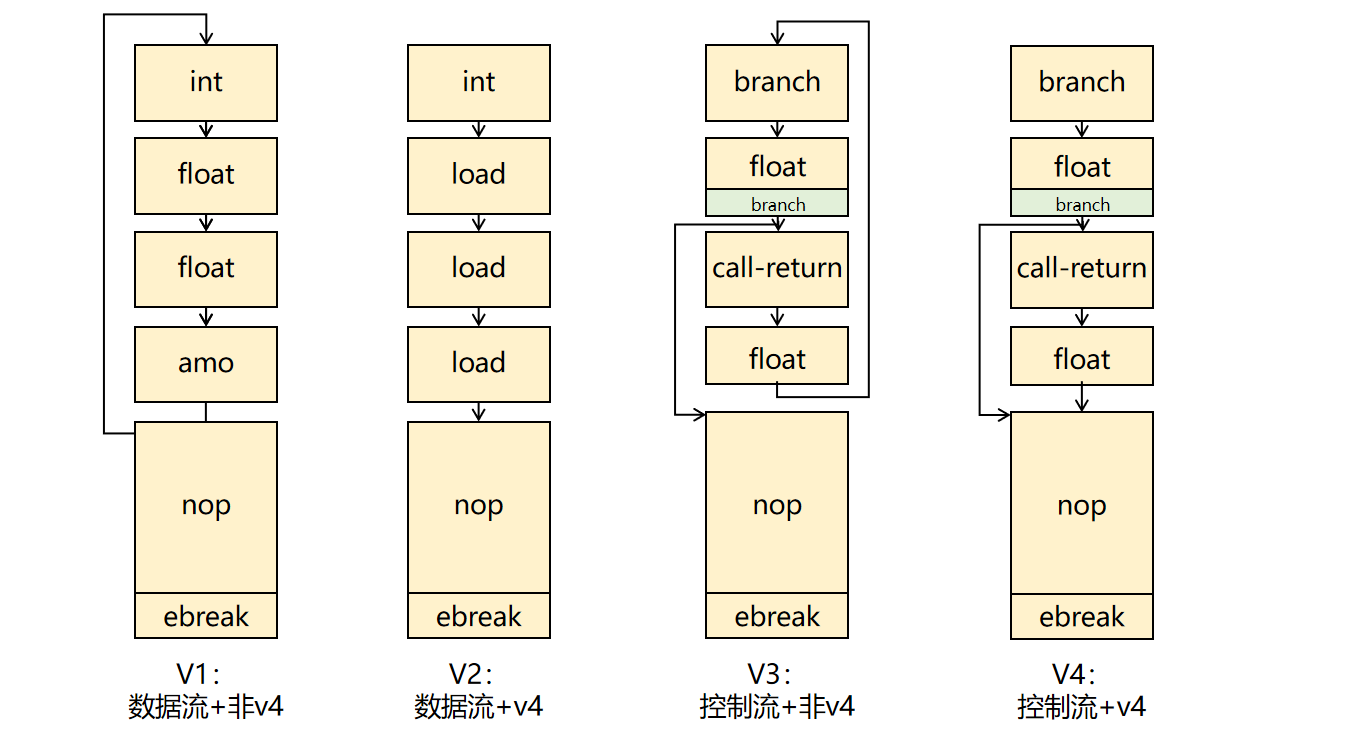
\includegraphics[width=\linewidth]{figure/paper/encode-consist.png}
    \caption{基本块控制流}
    \label{paper:encode-consist}
\end{figure}

\textbf{解码块(decode 块):}\par
decode 块和 encode 块配合使用,用于将 encode 编码在微架构状态中的 secret 利用时间侧信道解码出来。
考虑到在同样的地址执行同样的指令往往可以使用一样的微架构组件参与执行,
因此生成器简单的将 encode 块共用地址且相同的内容的代码块作为 decode 块。
需要注意的是,encode 块内部可能存在死循环,因此 decode 块需要将这个死循环打开。
此外 decode 块用 INFO\_LEAK\_START 和 INFO\_LEAK\_END 作为
decode 块的开始和结束,用于表示侧信道泄露秘密数据这一过程的开始和结束。\par

\textbf{替换块(replace 块):}\par
replace 块在 decode group 中被使用,用于替换 victim group 中 trigger 块、access\_secret 块的内容,
如果 trigger 块和 access\_secret 块的内容存在额外的 return 块,则需要将 return 块也替换掉。
因为 trigger 块和 return 块在这里不需要被使用,所以生成框架将 replace 块中的对应区域简单的替换为 nop 指令,
但是对于 access\_secret 块,后续的 decode 块需要从中得到和 secret 值相同的操作数,以此来复现 encode 块的指令执行,
所以 access\_secret 块的部分被替换为立即数构造 secret 值的简单代码。
这里需要注意的是,load\_init 块的指令和数据内部时携带了 return 块、access\_secret 块的 label,所以在生成 replace 块的时候
虽然已经将 return 块、access\_secret 块的内容替换为 nop,
但是需要保留它们的 label 信息且这些 label 要和 victim group 的 label 对齐,以确保 load\_init 块的数据保持不变。\par

\cleardoublepage
\section{评估及结果分析}

在本章节,我们对瞬态漏洞测试程序生成框架进行评估,以体现我们测试程序生成框架的高效性和高覆盖率。
对于瞬态窗口触发部分,我们对 train 块的三种变体进行测试,比较体现我们单条指令-地址敏感设计的有效性,
以及瞬态窗口触发类型挖掘的高覆盖率。随后我们对整体的瞬态漏洞测试程序生成进行评估,
通过统计挖掘完整瞬态漏洞 PoC 的时间开销和类型覆盖率,验证我们设计的高效性。
最后我们对特定的瞬态漏洞侧信道进行定向发掘,通过和 SpecDoctor 的挖掘时间进行横向对比,验证我们设计的高效性。\par

\subsection{评估环境和测试框架搭建}

为了进行 RISCV 处理器的仿真和测试,我们使用硬件修改后的开源处理器评估框架 starship 的作为测试平台,
使用 BOOM 处理器作为瞬态漏洞挖掘的开源 RISCV 处理器,使用 vcs 作为处理器仿真执行的综合工具。
本实验在 16 物理核,3.4GHz主频,128G内存的 AMD 5950X 服务器上进行测评。\par

测试框架有两阶段组成。阶段 1 如图\ref{paper:stage1-test}所示,首先随机产生一个测试框架代码块配置,
然后生成 train group、trigger group 的代码,执行 starship 平台的
BOOM 处理器仿真测试,如果检测到瞬态窗口触发就保存这个 trigger 样例,
进入下一阶段,不然就产生一组新的配置继续生成新的测试代码。
每轮迭代的配置和生成结果都会被暂存起来,供后续数据分析。\par

\begin{figure}[!h]
    \centering
    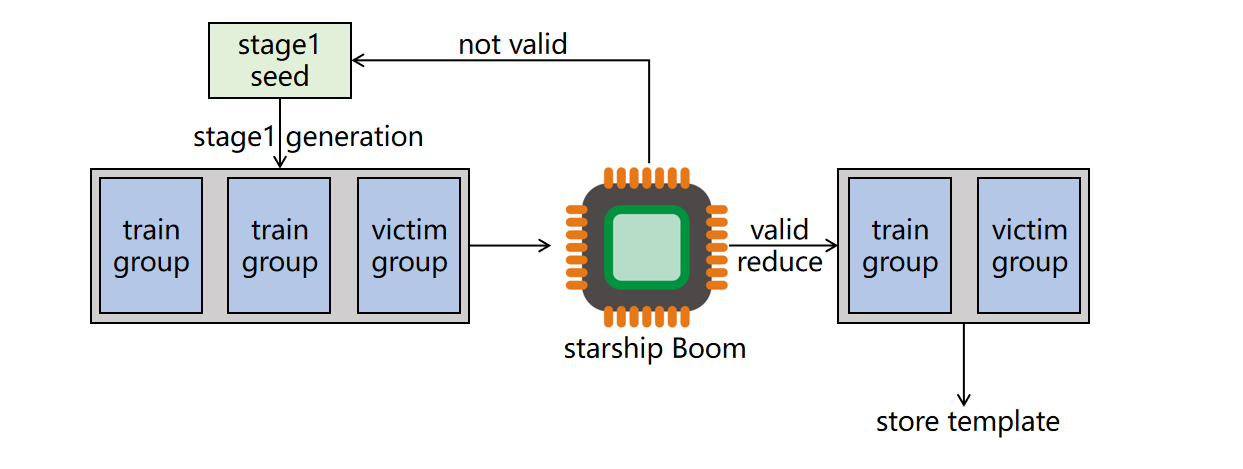
\includegraphics[width=\linewidth]{figure/paper/stage1-test.png}
    \caption{阶段1测试}
    \label{paper:stage1-test}
\end{figure}

阶段 2 如图\ref{paper:stage2-test}所示,在阶段 1 的 trigger 样例的基础上产生阶段二的代码块配置,
继而生成后续的 trans 部分和 decode group,然后在 starship 平台执行 BOOM 处理器的差分测试,
如果检测到执行时间不一致就保存这个 leak 样例。
每轮迭代的配置和生成结果都会被暂存起来,供后续数据分析。\par

\begin{figure}[!h]
    \centering
    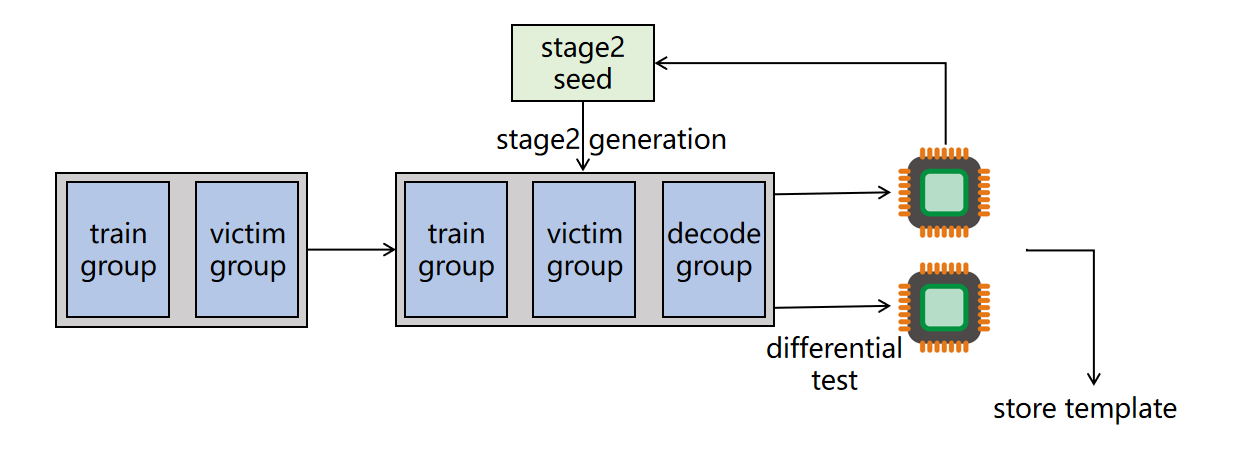
\includegraphics[width=\linewidth]{figure/paper/stage2-test.png}
    \caption{阶段2测试}
    \label{paper:stage2-test}
\end{figure}

\subsection{触发瞬态窗口效率评估}

为了检验生成框架使用单条指令-地址敏感的训练代码生成策略的有效性,我们分别使用 train 块的变体 V1(单条指令-地址对齐)、
V2(单条指令-地址不对齐)、V3(多条指令)生成 train 部分的代码,然后分别用 stage 1 测试框架进行 1 小时的测试,
然后对瞬态窗口触发程序生成的轮数、找到的瞬态窗口数、瞬态窗口类型占比等进行统计。\par

\subsubsection{测试结果分析}

V1、V2、V3进行一个小时测试之后,我们对各个变体找到的瞬态窗口类型进行统计。经过统计我们发现,train group 规约之后,trigger 指令
最多经过一个 train group 的训练就可以触发瞬态窗口,因此在表征触发瞬态窗口的类别时,我们使用 trigger 指令的类型和训练 trigger 指令的
train 指令的类型的组合进行表示。表\ref{table:v1-trans}、\ref{table:v2-trans}、\ref{table:v3-trans},
依次展示了 V1、V2、V3 找到的瞬态窗口种类、该类瞬态窗口的个数、该类瞬态窗口在大类中占比等信息。
后续我们将通过对 V1、V2、V3 的实验数据进行分析比较,验证我们训练策略的有效性。\par

V1 在单条指令、地址对齐的情况下测试 1 hour,共进行了 447 轮迭代,找到 228 个瞬态窗口。其中 jalr 跳转预测错误类型 5 类 67 个,
spectre-V4 存储预测错误类型 2 类 39 个,return 返回地址预测错误类型 2 类 35 个,branch 分支预测错误类型 3 类 30 个,
meltdown 异常延迟检测类型 6 类 57 个。其中通过训练触发的瞬态窗口共计 106 个。\par

\begin{table}[h!]
    \begin{center} 
    \caption{V1 瞬态窗口统计} 
    \label{table:v1-trans}  
    \resizebox{1.0\linewidth}{!}{
        \begin{tabular}{|l|l|l|l|l|l|l|l|} 
            \hline
            \textbf{trigger 类别} & \textbf{train 类别} & \textbf{窗口数} & \textbf{大类占比} & \textbf{trigger 类别} & \textbf{train 类别} & \textbf{窗口数} & \textbf{大类占比}\\
            \hline
            JALR                &TAKEN              &4  &5.97\%   &BRANCH              &NOT\_TAKEN         &11 &36.67\%  \\
            JALR                &JALR               &33 &49.25\%  &BRANCH              &NONE               &15 &50.00\%  \\
            JALR                &RETURN             &14 &20.90\%  &BRANCH              &TAKEN              &4  &13.33\%  \\
            JALR                &CALL               &13 &19.40\%  &STORE\_ACCESS\_FAULT&NONE               &10 &100.00\% \\
            JALR                &JMP                &3  &4.48\%   &STORE\_PAGE\_FAULT  &NONE               &12 &100.00\% \\
            V4                  &NONE               &34 &87.18\%  &STORE\_MISALIGN     &NONE               &3  &100.00\% \\
            V4                  &AMO                &5  &12.82\%  &LOAD\_ACCESS\_FAULT &NONE               &15 &100.00\% \\
            RETURN              &CALL               &31 &88.57\%  &LOAD\_PAGE\_FAULT   &NONE               &15 &100.00\% \\
            RETURN              &JALR               &4  &11.43\%  &LOAD\_MISALIGN      &NONE               &2  &100.00\% \\
            \hline
        \end{tabular}
    }
    \end{center}
\end{table}

V2 在单条指令、地址可以不对齐的情况下测试 1 hour,共进行了 453 轮迭代,找到 134 个瞬态窗口。其中 jalr 跳转预测错误类型 3 类 8 个,
spectre-V4 存储预测错误类型 4 类 37 个,branch 分支预测错误类型 1 类 26 个,
meltdown 异常延迟检测类型 6 类 63 个。其中通过训练触发的瞬态窗口共计 12 个。\par

\begin{table}[h!]
    \begin{center} 
    \caption{V2 瞬态窗口统计} 
    \label{table:v2-trans}  
    \resizebox{1.0\linewidth}{!}{
        \begin{tabular}{|l|l|l|l|l|l|l|l|} 
            \hline
            \textbf{trigger 类别} & \textbf{train 类别} & \textbf{窗口数} & \textbf{大类占比} & \textbf{trigger 类别} & \textbf{train 类别} & \textbf{窗口数} & \textbf{大类占比}\\
            \hline
            JALR                    &JALR     &3  &37.50\%   &BRANCH                  &NONE     &26 &100.00\%  \\
            JALR                    &RETURN   &4  &50.00\%   &LOAD\_MISALIGN          &NONE     &7  &100.00\%  \\
            JALR                    &CALL     &1  &12.50\%   &LOAD\_PAGE\_FAULT       &NONE     &12 &100.00\%  \\
            V4                      &NONE     &33 &89.19\%   &LOAD\_ACCESS\_FAULT     &NONE     &11 &100.00\%  \\
            V4                      &RETURN   &1  &2.70\%    &STORE\_MISALIGN         &NONE     &5  &100.00\%  \\
            V4                      &AMO      &2  &5.41\%    &STORE\_PAGE\_FAULT      &NONE     &12 &100.00\%  \\
            V4                      &STORE    &1  &2.70\%    &STORE\_ACCESS\_FAULT    &NONE     &16 &100.00\%  \\
            \hline
        \end{tabular}
    }
    \end{center}
\end{table}

V3 在多条随机指令的情况下测试 1 hour,共进行了 411 轮迭代,找到 120 个瞬态窗口。其中 jalr 跳转预测错误类型 1 类 2 个,
spectre-V4 存储预测错误类型 1 类 32 个,branch 分支预测错误类型 1 类 34 个,return 返回地址预测错误类型 1 类 1 个,
meltdown 异常延迟检测类型 6 类 51 个。其中通过训练触发的瞬态窗口共计 0 个。\par

\begin{table}[h!]
    \begin{center} 
    \caption{V3 瞬态窗口统计} 
    \label{table:v3-trans}  
    \resizebox{1.0\linewidth}{!}{
        \begin{tabular}{|l|l|l|l|l|l|l|l|} 
            \hline
            \textbf{trigger 类别} & \textbf{train 类别} & \textbf{窗口数} & \textbf{大类占比} & \textbf{trigger 类别} & \textbf{train 类别} & \textbf{窗口数} & \textbf{大类占比}\\
            \hline
            LOAD\_MISALIGN        &NONE &4  &100.00\% &            RETURN              &NONE &1  &100.00\%\\
            LOAD\_PAGE\_FAULT     &NONE &10 &100.00\% &            JALR                &NONE &2  &100.00\%\\
            LOAD\_ACCESS\_FAULT   &NONE &11 &100.00\% &            BRANCH              &NONE &34 &100.00\%\\
            STORE\_MISALIGN       &NONE &6  &100.00\% &            V4                  &NONE &32 &100.00\%\\
            STORE\_PAGE\_FAULT    &NONE &10 &100.00\% & & & & \\
            STORE\_ACCESS\_FAULT  &NONE &10 &100.00\% & & & & \\
            \hline
        \end{tabular}
    }
    \end{center}
\end{table}

\subsubsection{训练块生成策略对比}

\textbf{V1 与 V2 的对比:}
这里将单条指令对齐的训练块生成策略 V1 和单条指令不对齐的策略 V2 的测试结果进行对比,
以此体现训练指令地址敏感对于训练能力提高的重要性。
可以看到对于不需要训练的瞬态窗口触发类型,V1 和 V2 能找到相近个数的瞬态窗口,训练能力保持一致。
但是对于需要训练的瞬态窗口,V1 类型可以找到 10 种、共计 106 个瞬态窗口,
远远高于 V2 的 6 种、共计 12 个瞬态窗口。可以看到对于控制流类型的瞬态窗口触发指令,
例如分支预测错误、跳转目标预测错误、返回地址预测错误类型的 trigger 指令在训练时是地址极其敏感的,
有意识地让训练块进行地址对齐可以大大提高 trigger 指令训练的成功率。但是我们也可以看到 V2 找到了
两种 V1 没有找到的训练类型,即用 return 指令和 store 指令对 spectre-v4 进行训练,也许说明不对齐的 V2 变体
有时可以覆盖一些极其罕见的训练情况,故而 V2 变体在瞬态漏洞挖掘是可以作为 V1 的补充协同工作。\par

\textbf{V2 与 V3 的对比:}
这里将单条指令不对齐的训练块生成策略 V2 和 多条指令的训练块生成策略 V3 的测试结果进行对比,
以此说明训练指令条数的增加对于训练能力的提高意义不大,进而为单条指令训练的有效性提供依据。
可以看到 V3 类型因为产生的指令条目更多,训练代码更复杂,所以产生的测试程序更少,比 V2 少了 42 次迭代。
而无论是触发的瞬态窗口的种类,还是触发的瞬态窗口在迭代中的占比,V2 都和 V3 相近,甚至在这次测试中 V3 略低于 V2。
所以在多数情况下 V3 生成更多的训练指令并不能带来瞬态窗口触发上的收益,反而会降低测试程序生成的效率。
因此 V3 应该仅作为 V1 和 V2 的补充,而不能作为重要的生成策略。\par

\subsection{瞬态窗口类型介绍}

V1、V2、V3 收集到的瞬态窗口类型如表\ref{table:trans-summary}所示,这里我们对每种类型的机理进行简单介绍。\par

\begin{table}[h!]
    \begin{center} 
    \caption{瞬态窗口统计} 
    \label{table:trans-summary}  
    \resizebox{0.8\linewidth}{!}{
        \begin{tabular}{|l|l|l|} 
            \hline
            \textbf{瞬态窗口类别} & \textbf{预测部件} & \textbf{原理}\\
            \hline
            JALR+NONE               &   btb &   btb 默认预测错误      \\
            JALR+CALL/RETURN/JALR   &   btb &   jalr训练btb导致预测错误 \\
            JALR+TAKEN/NOT\_TAKEN/JMP&   btb &   jmp/branch训练btb导致预测错误 \\
            RETURN+CALL             &   rsb &   call训练rsb导致预测错误 \\
            RETURN+JALR             &   btb &   jalr训练btb导致预测错误 \\
            BRANCH+NONE             &   bim &   bim初始化值预测错误 \\
            BRANCH+BRANCH           &   bim &   branch训练bim导致预测错误 \\
            STORE\_PAGE\_FAULT      &   无  &   异常、权限延迟检测  \\
            STORE\_ACCESS\_FAULT    &   无  &   异常、权限延迟检测  \\
            STORE\_MISALIGN         &   无  &   异常、权限延迟检测  \\
            LOAD\_PAGE\_FAULT       &   无  &   异常、权限延迟检测  \\
            LOAD\_ACCESS\_FAULT     &   无  &   异常、权限延迟检测  \\
            LOAD\_MISALIGN          &   无  &   异常、权限延迟检测  \\
            V4                      &   lsu &   内存未修改预测错误  \\
            V4+AMO/STORE/return     &   lsu &   未知               \\
            \hline
        \end{tabular}
    }
    \end{center}
\end{table}

\textbf{JALR+NONE}的组合利用 jalr 指令的默认跳转目标预测。当 jalr 指令没有被训练时,
它在分支预测时查询对应的 btb 表,如果发现对应的 btb 表项正好为空,则默认选择跳转到 PC+4 的地址,
顺序执行下一条指令打开瞬态窗口。但是鉴于真实执行时处理器的 btb 表项大概率都已经有值了,
所以这个触发方式不容易发生。\par

\textbf{JALR+RETURN/CALL/JALR}的组合本质上是一样的,都是用 jalr 寄存器跳转指令训练寄存器跳转指令。
jalr指令在执行之后会将跳转的目标地址保存到处理器前端的 btb(branch target buffer)组件中,
然后在后续的 jalr 指令预测执行时会根据查找对应的 btb 表项得到预测的跳转地址,从而错误地进入瞬态窗口。
该类型就是在训练时用 jalr 指令跳转进入瞬态窗口地址,将瞬态窗口地址写入 btb,
使得 trigger 块的 jalr 错误的预测进入瞬态窗口。为了让训练的 jalr 指令和 trigger 块的 jalr
共用 btb 表项,所以这里的 jalr 指令需要地址对齐。\par

\textbf{JALR+JMP/TAKEN/NOT\_TAKEN}的组合也是用 jmp 指令和 branch 指令训练了 jalr 指令的 btb 表项,
但是 jmp 指令和 branch 指令的跳转地址本身其实不需要被预测,它们的跳转目标并不应该
修改 btb 表项,这侧面反映了 BOOM 的 btb 更新策略存在过度更新的漏洞。\par

\textbf{RETURN+CALL}的组合通过训练处理器的 RSB(return stack buffer)触发瞬态窗口。
call 指令执行时会将 pc+4 缓存到 rsb 中作为之后 return 指令的返回地址。我们只需要让
call 指令的下一条指令的地址是瞬态窗口的入口,return 指令预测执行的时候就会进入瞬态窗口。
这里的 call 和 return 指令并不需要地址对齐也可以触发这个机制。\par

\textbf{RETURN+JALR}的组合利用了 return 指令本身也是 jalr 指令的特性进行工作。这说明了 return 指令
并不仅仅根据 rsb 进行跳转地址的预测,在条件合适的情况下也可以使用 btb 中的数据进行分支预测。\par

\textbf{BRANCH+TAKEN/NOT\_TAKEN}的组合利用了 branch 指令对 branch 指令的训练。
当 branch 指令执行完毕后,它的跳转与否会被提交到 bim 组件中,之后 branch 再次执行时会检查 bim 部件
对应表项的跳转与否的预测,然后进行跳转。如果需要 branch 指令错误跳转进入瞬态窗口,
需要用 branch 指令将 bim 表项训练为 taken;如果希望 branch 指令错误不跳转进入瞬态窗口,则
需要用 branch 指令将 bim 表项训练为 not taken。为了让训练的 branch 和触发的 branch 共用一个 bim
表项,需要让它们地址对齐。\par

\textbf{BRANCH+NONE}的组合,因为 bim 表项在完成 bim 的初始化之后都会被初始化为 10,所以
即使不训练 branch 指令默认也是跳转的,所以如果需要错误预测跳转,不训练也可以触发。但是在
真实的场景下,处理器的 BIM 状态是随机的,还是需要 branch 指令将状态调整到可控的状态。\par

\textbf{STORE/LOAD + ACCESS\_FAULT/PAGE\_FAULT}的组合利用了处理器的异常延时检测技术。
这些指令不需要被训练,当处理器遇到这些指令时首先假设这些指令是满足权限的,然后后续的指令顺序执行。
在得到内存地址之后才开始进行权限的检测,因为权限的检测涉及到走页表、检查pmp寄存器需要比较长的时候,
所以当权限检测错误时又将长的窗口期可以触发瞬态执行漏洞。\par

\textbf{STORE/LOAD\_MISALIGN + NONE}的组合也利用了异常的演示检测。但是因为地址不对齐可以在得到内存地址之后
立刻进行判断,所以虽然也可以触发瞬态窗口,但是窗口期太短,
实际实验表明只有在极小概率下这个瞬态窗口才可以支持后续的泄露秘密数据的操作。\par

\textbf{V4+NONE}的组合利用了内存载入部件 lsu 的预测错误。当进行内存访问时,后执行的 load 指令
假设之前发射的指令没有对需要访问的内存地址进行了修改,直接访问内存获得数据。但是之前发射的 store 指令
在 load 之后修改了该地址的内存,导致 store 之后的指令被回滚,进而打开了瞬态窗口。该指令也不需要训练就可以触发。\par

\textbf{V4+AMO/RETURN/STORE}的组合,这是本工作发现的全新的训练组合,
在之前的研究中并没有提到 V4 类型需要被额外训练才可以生效,是本工作的全新发现,
但是具体训练的机制未知,有待后续进一步的研究。\par

根据表\ref{table:trans-summary}可以看到,我们的瞬态漏洞测试程序生成框架在 1 小时内就可以找到 15 种类型的
瞬态窗口,包含了 spectre V1-V4、ret-spectre、meltdown 类型的基本瞬态窗口类型,还发现了‘V4+AMO/STORE/RETURN’的未知情况。
充分证明了我们的生成框架在瞬态窗口的触发上有较高的生成效率和覆盖率。\par

\subsection{完整 PoC 生成评估}

为了验证生成框架生成完整 PoC 的能力和效率,我们让测试框架连续执行完整的 stage1 和 stage2 测试。stage1 执行得到的代码会被
送入 stage2 生成秘密访问和秘密泄露的代码,如果通过差分测试就会被保存起来。因为触发瞬态窗口和秘密泄露是相对独立的两部分代码,
所以 stage1 得到的代码可以被反复用于 stage2 的代码生成,因此我们让 stage1 得到的每个代码就被用于 20 次 stage2 代码的生成,
以提高 trigger 代码的利用率,并分摊 trigger reduce 的时间开销。
如此我们让生成框架进行 4 小时的测试,然后分析总结得到的泄露秘密数据的类别和数目。为了可以和 SpecDoctor 的随机代码生成方法进行横向对比,
我们采用和 SpecDoctor 一样的固定触发类型、泄露通道,再进行定向测试程序生成,将我们生成框架的漏洞触发时间和 SpecDoctor 进行横向比较。\par

\subsubsection{泄露秘密数据效率评估}

通过四个小时的测试,生成框架一共进行了 3599 次测试,找到了 166 个完整的 PoC,平均 21 次生成可以找到一个有效的 PoC。
因为 PoC 的泄露机制比较繁琐驳杂,需要进行人工的一一审核,在这里无法对所有 166 个 PoC 的泄露机制进行分门别类,所以
仅对一些有代表性的 PoC 泄露机制进行简要介绍,以佐证我们实验的真实性和完整性。\par

\textbf{低位匹配泄露 secret 数据:}
access\_secert 块在使用高位地址被随机数替换的地址进行内存访问,获得 secret 值时,仍然可以成功获得 secret。实验表明
这首先需要 secert\_migrate 块将数据载入到 cache 或者 load buffer,然后因为 buffer 匹配时只使用地址的一部分(高位用于权限验证),
所以仅当低位匹配时,access\_secert 块就可以从 cache 或者 load buffer 获得 secret 的值。在成功的 PoC 中高位替换的地址最多在
替换了高 24 位之后依然可以有效匹配,所以 BOOM 的 buffer 使用的匹配地址最多不出超过 40 位。\par

\textbf{通过 cache 侧信道泄露:}
代码样例如图\ref{code:cache-channel}所示,其中 secret 数据被保存在 s0 寄存器中,本体的 secret 值为 101,变体的 secret 值为 0。
当执行该代码时,本体访问地址 channel\_page\_base\_0 + 96 + 0x5c8 和 channel\_page\_base\_0 + 96 + 0x5e8 所在的内存,
将这部分数据带入 cache;而变体将 channel\_page\_base\_0 + 0x5c8 和 channel\_page\_base\_0 + 0x5e8 的数据带入 cache。
当 decode group 重新执行这部分代码是,因为 s0 的值在本体变体都是 101,所以访问地址  channel\_page\_base\_0 + 96 + 0x5c8 和 channel\_page\_base\_0 + 96 + 0x5e8 。
因为本体可以在访问时命中 cache 所以执行速度比较快,但是变体因为 cache miss,执行速度比较慢,从而产生时间侧信道的差异,导致秘密的泄露。\par

\begin{figure}[htbp]
    \centering
    \begin{minted}{c}
        la a1, channel_page_base_0
        andi s0, s0, 0x7f8
        add a1, a1, s0
        flw ft3, 0x5c8(a1)
        ld a7, 0x5e8(a1)
    \end{minted}
    \caption{用cache泄露秘密数据}
    \label{code:cache-channel}
\end{figure}

\textbf{通过阻塞流水线:}
代码样例如图\ref{code:port-stall}所示。因为变体的 s0 等于 0,而本体的等于 101,所以本体会执行这个循环的浮点指令,而变体不会。
当瞬态窗口撤销时,本体发射的浮点指令还在 FPU 中执行无法直接从 FPU 中撤销,所以流水线必须等待 FPU 中的浮点指令执行完毕才可以
回滚瞬态窗口,这导致变体可以比本体提前执行结束。
所以通过阻塞流水线产生了时间差异,进而泄露了 secret 数据。\par

\begin{figure}[htbp]
    \centering
    \begin{minted}{c}
        encode_block_0:
            c.beqz s0, encode_nop_fill
            fsgnj.d ft3, ft8, ft2
            fmsub.d fs10, ft7, ft11, ft9
            fmax.s ft10, fs6, fs6
            fclass.d gp, fs8
            fsub.s ft2, fs1, fs11
            fcvt.d.wu fs1, a5
            fsgnj.s fa3, ft5, ft1
            jal zero, encode_block_0
        encode_nop_fill:
    \end{minted}
    \caption{用阻塞流水线泄露秘密数据}
    \label{code:port-stall}
\end{figure}

\textbf{通过BIM预测器:}
代码样例如图\ref{code:bim-channel}所示。可以看到本体会执行分支中的 branch 指令,但是变体不会。
当 branch 指令被执行时,bim 模块内部的状态被修改,之后 decode group 执行时本体因为预测的存在可以执行得更快,
但是变体则相对较慢,从而泄露了秘密数据。但是 BOOM 承诺瞬态窗口执行的 branch 的预测结果是不会更新 bim 的,
因此这也暗示了 bim 的更新逻辑存在 bug。\par

\begin{figure}[htbp]
    \centering
    \begin{minted}{c}
            c.beqz s0, encode_nop_fill
        encode_block_1:
            bge s10, a7, encode_block_1_1
        encode_block_1_1:
            blt t0, s4, encode_block_1_2
        encode_block_1_2:
            bltu t0, sp, encode_block_1_3
        encode_block_1_3:
            beq s7, t3, encode_block_1_4
        encode_block_1_4:
            bge s11, s7, encode_block_1_5
        encode_block_1_5:
            bgeu a7, s6, encode_block_1_6
        encode_nop_fill:
    \end{minted}
    \caption{用BIM泄露秘密数据}
    \label{code:bim-channel}
\end{figure}

其他 PoC 也有利用 rsb、btb 等组件进行秘密数据泄露的,另外也包括一些原理不明的 PoC 程序有待后续的进一步分析归类。故而
我们的秘密数据泄露 PoC 至少覆盖了 cache、btb、bim、rsb、port 五个侧信道。\par

\subsubsection{SpecDoctor 的横向比较}

这里我们固定了触发瞬态窗口的机制和泄露秘密数据的侧信道,进行定向的 PoC 生成,然后将我们找到第一个 PoC 所使用的时间
和 SpecDoctor 论文使用的时间进行对比,通过横向比较衡量我们生成框架的性能。测试结果如表\ref{table:cmp-specdoctor}所示。
可以看到 SpecDoctor 因为使用随机的指令生成方式,所以每个 PoC 生成所需的时间都是 10hour 级别的,
而我们使用策略生成+地址敏感测试程序仅仅需要 1-3 min 就可以得到需要的 PoC,这也充分验证了我们生成策略的高效性。\par

\begin{table}[h!]
    \begin{center} 
    \caption{与 SpecDoctor 的性能比较} 
    \label{table:cmp-specdoctor}  
    \resizebox{0.7\linewidth}{!}{
        \begin{tabular}{|l|l|l|l|} 
            \hline
            \textbf{瞬态窗口类型} & \textbf{泄露通道} & \textbf{本框架用时} & \textbf{SpecDoctor 用时}\\
            \hline
            load\_page\_fault   &   dcache      &   2m24s   &   34.7h   \\
            store\_page\_fault  &   dcache      &   1m9s    &   46.1h   \\
            branch\_mispredict  &   dcache      &   2m31s   &   30.6h   \\
            branch\_mispredict  &   front-end   &   2m31s   &   31.2h   \\
            \hline
        \end{tabular}
    }
    \end{center}
\end{table}

\cleardoublepage
\section{不足与展望}

虽然相比与现在的一些瞬态测试程序生成工作,本生成框架有更高的生成效率和覆盖率,但是仍有许多不足和改进的空间。

\begin{enumerate}
    \item 本生成框架暂不支持使用 csr 指令、rocc 指令、密码学扩展指令、fence 指令等进行训练,在指令的覆盖率上可以进一步扩展。
后续可以考虑为处理器提供 rocc 部件和密码学计算部件,来增加这些指令的场景;对于 csr 指令的修改做一些调整和约束,确保在修改 csr
指令的同时不会破坏程序的正常执行。\par
    \item 本生成框架没有考虑瞬态窗口出现在异常处理程序的情况,故而控制流预测进入异常处理程序的情况会被测试程序忽略掉。
当测试程序发生异常进入异常处理程序时,可能前端的控制流预测组件也会记录这些信息,从而在特定情况下预测进入异常处理程序。
但是生成框架暂时没有对异常处理程序进行插桩和瞬态窗口填充的支持,因此暂时假定瞬态窗口不会在异常处理程序出现。\par
    \item 本生成框架主要考虑的是前端控制流预测错误的情况,对于类似 V4 变体数据流预测错误的情况并没有很好的设计和覆盖。
V4 启示我们并不仅仅只有控制流会发生预测,内存的访问、计算单元的计算结果都可能是预测产生的,因此我们既要考虑控制流预测的情况,
也应该考虑数据流预测的情况,包括发生数据流预测错误如何设置瞬态窗口、如何防止秘密数据被显式访问等。\par
    \item 本生成框架暂时不支持中断发生的情况。如果中断发生也可能对处理器的执行情况进行改变,进而影响处理器控制流的预测、微架构的编码
等,对于瞬态窗口触发和秘密数据泄露也许都会有影响。因此需要提供通过监视处理器内部执行情况触发外部中断的机制,让中断在合适的时机发生。\par
    \item 本生成框架在瞬态漏洞定位方面存在不足。虽然生成框架可以产生 PoC,但是 encode 块内部的代码过于繁多和驳杂,依靠手动定位和
分析过于费时费力,所以需要一个简单有效的机制过滤掉 encode 块中的冗余代码,将搜索空间变得尽可能小,进而提高漏洞定位的效率。\par
    \item 本生成框架仅在 BOOM 处理器上进行测试验证,对于 xiangshan 等其他乱序处理器、大型商用处理器都没有进行验证考量,
其生成功能的通用性、泛化性还有待更多实验的验证。\par
\end{enumerate}

\cleardoublepage
\section{总结}

本文提出了一种适用于 RISCV 处理器的瞬态执行漏洞发掘的高效测试程序生成框架。
该框架可以支持物理态、内核态、用户态的执行,支持虚拟地址和物理地址的执行,支持 rv64imafdc 的全集和 zicsr 扩展的子集。
为了解决现有瞬态执行漏洞测试生成框架随机生成的低效性问题,我们采用操作数约束执行、代码块策略生成、
地址敏感的训练代码和泄露代码排布、物理内存切换等技术进行解决。该生成测试框架可以在 4 小时内找到 166 个 BOOM 处理器的完整 PoC,
覆盖 15 种瞬态窗口类型和至少 5 种侧信道,对于给定的窗口类型和侧信道类型可以在 min 的时间量级内找到 PoC,远快于 SpecDoctor 等
随机生成框架的 hour 级别。\par
